\documentclass[11pt,]{article}
\usepackage[]{mathpazo}
\usepackage{amssymb,amsmath}
\usepackage{ifxetex,ifluatex}
\usepackage{fixltx2e} % provides \textsubscript
\ifnum 0\ifxetex 1\fi\ifluatex 1\fi=0 % if pdftex
  \usepackage[T1]{fontenc}
  \usepackage[utf8]{inputenc}
\else % if luatex or xelatex
  \ifxetex
    \usepackage{mathspec}
  \else
    \usepackage{fontspec}
  \fi
  \defaultfontfeatures{Ligatures=TeX,Scale=MatchLowercase}
\fi
% use upquote if available, for straight quotes in verbatim environments
\IfFileExists{upquote.sty}{\usepackage{upquote}}{}
% use microtype if available
\IfFileExists{microtype.sty}{%
\usepackage{microtype}
\UseMicrotypeSet[protrusion]{basicmath} % disable protrusion for tt fonts
}{}
\usepackage[margin=1in]{geometry}
\usepackage{hyperref}
\hypersetup{unicode=true,
            pdfborder={0 0 0},
            breaklinks=true}
\urlstyle{same}  % don't use monospace font for urls
\usepackage{longtable,booktabs}
\usepackage{graphicx,grffile}
\makeatletter
\def\maxwidth{\ifdim\Gin@nat@width>\linewidth\linewidth\else\Gin@nat@width\fi}
\def\maxheight{\ifdim\Gin@nat@height>\textheight\textheight\else\Gin@nat@height\fi}
\makeatother
% Scale images if necessary, so that they will not overflow the page
% margins by default, and it is still possible to overwrite the defaults
% using explicit options in \includegraphics[width, height, ...]{}
\setkeys{Gin}{width=\maxwidth,height=\maxheight,keepaspectratio}
\IfFileExists{parskip.sty}{%
\usepackage{parskip}
}{% else
\setlength{\parindent}{0pt}
\setlength{\parskip}{6pt plus 2pt minus 1pt}
}
\setlength{\emergencystretch}{3em}  % prevent overfull lines
\providecommand{\tightlist}{%
  \setlength{\itemsep}{0pt}\setlength{\parskip}{0pt}}
\setcounter{secnumdepth}{0}
% Redefines (sub)paragraphs to behave more like sections
\ifx\paragraph\undefined\else
\let\oldparagraph\paragraph
\renewcommand{\paragraph}[1]{\oldparagraph{#1}\mbox{}}
\fi
\ifx\subparagraph\undefined\else
\let\oldsubparagraph\subparagraph
\renewcommand{\subparagraph}[1]{\oldsubparagraph{#1}\mbox{}}
\fi

%%% Use protect on footnotes to avoid problems with footnotes in titles
\let\rmarkdownfootnote\footnote%
\def\footnote{\protect\rmarkdownfootnote}

%%% Change title format to be more compact
\usepackage{titling}

% Create subtitle command for use in maketitle
\newcommand{\subtitle}[1]{
  \posttitle{
    \begin{center}\large#1\end{center}
    }
}

\setlength{\droptitle}{-2em}
  \title{}
  \pretitle{\vspace{\droptitle}}
  \posttitle{}
  \author{}
  \preauthor{}\postauthor{}
  \date{}
  \predate{}\postdate{}

\usepackage{lineno}
\linenumbers

\begin{document}

\section{\texorpdfstring{Elahi \emph{et al.} - Supporting
information}{Elahi et al. - Supporting information}}\label{elahi-et-al.---supporting-information}

\subsection{WebPanel 1. Methods}\label{webpanel-1.-methods}

\subsubsection{Processing the raw AIS
data}\label{processing-the-raw-ais-data}

We used vessel positioning data to infer the spatial distribution of
trawling effort in the Adriatic Sea. Specifically, we used Automatic
Identification System (AIS) data for the Adriatic Sea from 1 January
2014 to 31 July 2016. In Europe (EU Dir 2011/15/EU), all fishing vessels
greater than 15m in length are required to use AIS transmitters. The AIS
data were provided by \emph{NAVAMA} (\url{http://navama.com/}), and were
based on both terrestrial and satellite (Orbcomm,
\url{https://www.orbcomm.com/}) receivers. In a separate study, the
spatial coverage of terrestrial receivers was observed to be between
75-100\% throughout the Adriatic Sea (Vespe \emph{et al.} 2016),
suggesting that AIS data in this region is reliable; no spatial biases
due to incomplete coverage were apparent in our analyses.

The raw vessel position dataset (n = 11,616,639 records) included all
Adriatic vessels that listed primary or secondary gears with demersal
effects (i.e., bottom trawls, beam trawls, dredges) in the fleet
register of the European Union (Eurostat 2016). The filtering steps of
the raw vessel position data followed the recommendations of Hintzen
\emph{et al.} (2012) and are summarized in WebTable 1.

After filtering, the number of unique bottom trawlers was 2, 3, 92, and
549 for Albania, Slovenia, Croatia, and Italy, respectively. By
comparison, the number of vessels with bottom trawl gear listed as
primary gear in the EU fleet register (2014-2016) was 5, 169, and 956
for Slovenia, Croatia, and Italy, respectively. Across these three
countries, the median vessel size was 14.8m. When we limited the Italian
fleet to vessels registered in Adriatic ports, the number of Italian
vessels dropped to 506, and the median size for Adriatic vessels was
13.9m. This suggests that we had AIS coverage for all Italian vessels
registered in the Adriatic, and an additional 43 Italian vessels
registered elsewhere (e.g., the Ionian Sea). Due to licensing
restrictions with our data partner NAVAMA, we were not permitted
information on port of registration (or any other characteristics beside
gear type) for the vessels in our AIS dataset. When we limited the fleet
register to vessels greater than 15m in length (at which AIS is required
for EU vessels), the number of trawlers declined to 2, 63, and 179 for
Slovenia, Croatia, and Italy, respectively. In summary, our AIS dataset
contained 646 vessels and the Adriatic fleet register listed 680
vessels, suggesting that we captured nearly all of trawlers in the
Adriatic Sea, and virtually all of the large (\textgreater{}15 m)
vessels. These large vessels catch disproportionately more fish, and are
more likely to travel further offshore (e.g., the Jabuka-Pomo Pit).

All commercial fishing vessels in the European Union are registered in a
port, but many vessels land fisheries catches, or otherwise visit, other
ports. Due to this complication, if we wish to understand port-scale
estimates of fishing effort, we must first (1) identify individual
vessel trips and then (2) associate each trip to a port of origin and/or
a port of destination.

\paragraph{Identifying vessel trips}\label{identifying-vessel-trips}

Following methods in Bertrand \emph{et al.} (2005), trips were defined
as a series of records at sea bounded by in-port positions. If there
were more than two consecutive in-port pings, we first removed
intermediate positions - and thus the first in-port positions served as
the previous trip's destination, and the last in-port position served as
the next trip's starting position. We then calculated the interval
between positions (in minutes); the median interval was 12 minutes. Next
we removed pseudoduplicate vessel positions (Hintzen \emph{et al.}
2012), which were defined as positions with a very short time interval
from the past position (\textless{}1 minute), and recalculated the time
interval. These positions were likely due to errors in AIS transmission
and do not provide critical spatial information because movement is
minimal in such a short span of time.

The time interval between positions was also used to define vessel trips
because it was apparent from the data that the starting or ending
in-port position was not detected for every vessel trip. Therefore, it
was necessary to define a threshold for the interval between positions
to designate new trips. This threshold needed to balance the risk of
falsely detecting a starting position (i.e., Type I error) against not
detecting a true starting position (i.e., Type II error). The
consequences of these two errors, respectively, are splitting a single
true trip into multiple apparent trips versus creating artifactually
long trips by combining multiple true vessel trips into a single,
apparent trip. We chose to use an interval threshold of 12 hours. A
computational experiment demonstrated that the use of 12 hours was a
reasonable minimum, because the maximum trip duration and the percent of
trips shorter than 120 hours (5 days) approached their asymptotes by
\textasciitilde{}12 hours (WebFigure 1). Five days is a relevant
duration because most Italian trawling vessels are not permitted to
operate on weekends. Nevertheless, the specific choice of interval does
not influence the remainder of our analyses, as we focus on aggregate
metrics of fishing effort (e.g., region, port, or vessel).

\paragraph{Identifying destination ports for each vessel
trip}\label{identifying-destination-ports-for-each-vessel-trip}

After the identification of individual vessel trips, it was necessary to
associate each trip with a specific port. In the best-case scenario, the
first and last vessel position for a given trip was located within a
port (54.2\% of trips); we will refer to these positions as the trip
origin and trip destination, respectively. We chose to focus on the trip
destination as the assigned port for each trip, because the destination
is most relevant for catch landings. However, some trips lacked a
destination for port assignment. In these cases, we applied the
following set of rules to assign a port.

If the trip destination was missing, we used the next trip's port of
origin if it matched the trip origin - resulting in a total of 63.2\% of
trips with an assigned port of destination. If the trip origin was
missing, or it did not match the next trip's port of origin, we used the
next trip's port of origin (68.3\% of trips with port). If the latter
was missing, then we assigned the trip destination to the most recent
destination port - but only if the immediate future trip destination was
the same (92.0\% of trips with port). Finally, if the most recent trip
destination differed from the following trip destination, the more
probable (i.e., the one with the highest frequency) of the two ports was
selected. Therefore the only trips unassigned a port destination were
for vessels lacking in-port positions entirely; 99.2\% of trips were
assigned a destination port.

\paragraph{Identifying fishing
activity}\label{identifying-fishing-activity}

Once the raw data were cleaned and filtered, we classified the remaining
points as fishing or not. Although simple speed filters can be effective
for identifying trawling activities (Murawski \emph{et al.} 2005), we
chose to apply a more restrictive approach based on the individual speed
profiles for each vessel. Specifically, we used segmented regression to
identify the lower and upper break points for the peak of the speed
distribution after the application of a preliminary speed filter of 0.5
to 8 knots (Hintzen \emph{et al.} 2012). Occasionally, the segmented
regression identified relatively high speeds as fishing positions, but
we restricted fishing positions to \(\leq\) 4 knots (Lee \emph{et al.}
2010; Russo \emph{et al.} 2013). Similarly, when the segmented
regression failed due to low sample size (0.007\%), we classified
vessels as fishing when their speeds were \(\leq\) 4 knots. This dataset
of fishing positions was then used to calculate the number of fishing
hours per \textasciitilde{}2.4km\textsuperscript{2} grid cell (0.016
longitude × 0.016 latitude) in the study area (defined below).

\subsubsection{Defining the study period and
area}\label{defining-the-study-period-and-area}

The Jabuka-Pomo closure began officially on 25 July 2015, but for
simplicity we defined `before closure' and `after closure' periods as
August 2014-July 2015 and August 2015-July 2016, respectively. The total
number of vessels observed to be trawling in the Adriatic Sea was 608
and 599 for before and after periods, respectively. Due to the large
spatial extent of the complete dataset, not all of the trawling effort
in the Adriatic Sea was likely to be affected, directly or indirectly,
by the spatial closure. Therefore, we needed to define a relevant study
area in the central Adriatic Sea.

First, we identified vessels that were likely to be impacted
disproportionately by the spatial closure. For each vessel, we
calculated the number, and percentage (of total), of fishing hours
inside the borders of the spatial closure in the year prior to the
trawling ban. Vessels that exhibited fishing effort greater than the
95\textsuperscript{th} percentile, in total hours and percentage of
total hours, were defined as `impacted' (n = 22; WebFigure 2). We
removed 14 grid cells that were exceptionally far from the Jabuka-Pomo
closure (\textgreater{} 130 km; WebFigure 3). The removed data
represented 0.6\% of the total fishing effort for one impacted vessel
from San Benedetto del Tronto. Although it is interesting that this
single vessel fished further after the trawling ban, we sought to
understand the general consequences of the Jabuka-Pomo closure and thus
we deemed it appropriate to modify the spatial domain (WebFigure 4) of
the impacted vessels in this way.

Second, the spatial domain of these impacted vessels was used to
identify control vessels. As a primary criterion, control vessels were
restricted to fishing within the spatial domain of the impacted vessels.
In addition to this primary criterion, vessels that fished minimally
(\textless{} 5\%) in the Jabuka-Pomo closure, and minimally in total
(\textless{} 5\textsuperscript{th} percentile of total fishing hours)
prior to the trawling ban were identified as `control' (n = 31).

Any remaining vessels that fished inside of the defined study area were
defined as `other' vessels (n = 316). These other vessels were either
vessels that fished exclusively in the study area but exhibited
displacement values intermediate to control and impacted vessels (e.g.,
\textgreater{} 5\%), or vessels that fished inside and outside the study
area. The fishing effort inside of the study area is presented for each
of these three categories of vessels in WebFigure 5.

\subsubsection{Data analysis}\label{data-analysis}

To visualize the redistribution of fishing effort after the trawling
ban, we calculated the log change in fishing effort for grid cells,
ports, and vessels in the study area. We added the 1\textsuperscript{st}
percentile of non-zero fishing effort to all of the cells (0.27 hours)
and ports (0.23 hours), and then calculated the change in fishing effort
as (\(log_{10}\){[}\(hours_{after}\)/\(hours_{before}\){]}). For ports,
we calculated the total fishing effort inside of the study area, but our
interpretations are unchanged if we calculate port effort across the
entire Adriatic. Only ports in the 75th percentile of fishing hours are
displayed on the map (Figure 2a) for clarity. To further visualize the
scale-dependence of changes in effort redistribution, we examined
qualitatively whether total effort changed after the closure for control
and impacted vessels. To facilitate the illustration of general trends
in vessel-scale changes in effort, two negative outliers (control
vessels that did not fish at all after the trawling ban) were removed
from the plot, but were used in the calculation of the boxplot
statistics (e.g., the median). These two outliers represented a
\(log_{10}\) change of \textasciitilde{}2 and \textasciitilde{}3 (10 and
100-fold reduction). In the boxplots of log change in effort (Figure 2b,
2d) the whiskers reach up to 1.5 times the interquartile range and
outliers are displayed as gray points.

We modeled statistically the redistribution of fishing effort in the
context of several hypothesized predictors. \emph{A priori}, we expected
that fishing effort would be affected by distance from the Jabuka-Pomo
border, distance from shore, depth, bottom slope, and habitat quality
(WebFigure 6, 7). Distance to the Jabuka-Pomo border was calculated for
each grid cell as the straight-line distance. Distance to shore, depth,
and bottom slope for each grid cell was retrieved from Sbrocco and
Barber (2013).

We defined habitat quality in reference to the persistence of nursery
grounds, using data for five commercially exploited species in the study
area (Colloca \emph{et al.} 2015). In brief, Colloca \emph{et al.}
(2015) used time series of scientific trawls to identify spatial
hotspots of fish nurseries in the Mediterranean Sea, and developed an
index of persistence (across years) for each species. Persistence ranged
between 0 (cell \emph{i} never included in an annual nursery hotspot)
and 1 (cell \emph{i} always included in an annual nursery hotspot), and
was reported as an ordinal value from 1-5 (representing 0.05-0.20,
0.21-0.40, 0.41-0.60, 0.61-0.80, and 0.81-1.0). Habitat quality was then
defined as the sum of persistence, for all species \emph{j}, in each
grid cell \emph{i}:

\[Habitat\ quality_{i} = \sum_{j=1}^{n}Persistence_{i}\]

We used a generalized additive model (GAM) to understand the predictors
of fishing effort (in hours) because we did not expect all of the
covariates to be related linearly to the dependent variable. Namely, we
expected fishing hours to display non-linear (i.e., smoothed) responses
to the distance from the Jabuka-Pomo border, distance from shore, and
depth. In contrast, we included habitat quality and bottom slope as
linear terms. We also included longitude and latitude as a smoothed term
in order to account explicitly for spatial position. All smoothed terms
were fit using thin plate regression splines. We used a gamma
distribution because fishing hours cannot be negative, and the variance
of fishing hours was assumed to increase with the mean. The model is
given by:

\[Effort_{i} = Gamma(\mu_{i}, \tau)\] \[E(Effort_{i}) = \mu_{i}\]
\[var(Effort_{i}) = \frac{\mu^{2}_{i}}{\tau}\]
\[log(\mu_{i}) = \alpha + \beta_{p}Period_{i} + \sum_{l=1}^{n}\beta_{l_{1}}Covariate_{i} + \sum_{l=1}^{n}\beta_{l_{2}}Covariate_{i}Period_{i} ~+\]
\[f_{s}(Long_{i}, Lati_{i}) + \sum_{s=1}^{n}f_{s}(Covariate_{i},Period_{i})\]
where effort in grid cell \emph{i} is related to the intercept
(\(\alpha\)), linear covariates (\(\beta\)), and smoothed covariates
(\(f_{s}\)) by each period (before and after the closure). The expected
values of \(Effort_{i}\) are \(\mu_{i}\) with a quadratic variance;
\(\tau\) is estimated from the data and controls the shape of the gamma
distribution. We used the function \texttt{bam()} from the package
\texttt{mgcv} (Wood 2006) in R 3.4.0 (R Core Team 2017) to fit the GAM.

Distance to the closure border was correlated strongly with depth (r =
-0.69, WebFigure 8), and the variance inflation factor for depth was
2.3. Therefore we removed depth from our model, and the variance
inflation factors for all remaining terms were \textless{} 2 (Zuur
\emph{et al.} 2010). We did not employ a model selection approach
because all of the covariates in our model were selected to test
specific hypotheses based on our understanding of the behavior of
fishers in general, and trawlers specifically. Rather than use a
data-mining approach to find a subset of covariates that composed a
`best' model, we opted to include all of our original covariates and
make inferences based on significance tests conditional on the full
model. Due to the signal of spatial autocorrelation that remained after
accounting for the spatially explicit nature of the data (using a
smoothed term for latitude and longitude), we caution against inferring
meaningful effects associated with p-values bordering on significance
(e.g., close to 0.05). However, none of the significance tests were
questionable. Beyond 10km, the signal of spatial autocorrelation was
minimal (WebFigure 9).

All of the data and R scripts necessary to reproduce the analyses will
be uploaded to the Stanford Digital Repository prior to publication.

\newpage

\subsection{WebTable 1. List of the steps used for filtering the raw
vessel position
data}\label{webtable-1.-list-of-the-steps-used-for-filtering-the-raw-vessel-position-data}

\begin{longtable}[]{@{}llr@{}}
\toprule
& Processing step & Rows (n)\tabularnewline
\midrule
\endhead
1 & Raw data & 11616639\tabularnewline
2 & Removed duplicated records & 11614737\tabularnewline
3 & Selected vessels with otter trawl as primary gear &
10882826\tabularnewline
4 & Removed intermediate port pings & 9843127\tabularnewline
5 & Removed pseudoduplicates & 9724023\tabularnewline
6 & Removed intermediate long interval pings & 9714351\tabularnewline
7 & Removed single ping trips & 9713845\tabularnewline
8 & Applied preliminary speed filter (0.5 - 8 knots) &
8436974\tabularnewline
9 & Removed in-port pings & 8261811\tabularnewline
10 & Selected points in Adriatic & 8235794\tabularnewline
11 & Removed coastal pings (\textless{} 3 nm) & 7663419\tabularnewline
12 & Selected fishing points & 3606738\tabularnewline
\bottomrule
\end{longtable}

\newpage

\subsection{\texorpdfstring{WebTable 2. Results of a generalized
additive model testing the effects of distance variables, habitat
quality, and bottom slope by the timing of the Jabuka-Pomo closure on
the number of fishing hours (log) per grid cell. Linear parameters are
presented with the estimate, 95\% confidence interval (CI), t-value
(\emph{t}), and p-value (\emph{P}); smoothers are presented with the
effective degrees of freedom (DF), f-statistic (\emph{F}), and p-value
(\emph{P}). See WebFigure 10 for a visualization of these
estimates.}{WebTable 2. Results of a generalized additive model testing the effects of distance variables, habitat quality, and bottom slope by the timing of the Jabuka-Pomo closure on the number of fishing hours (log) per grid cell. Linear parameters are presented with the estimate, 95\% confidence interval (CI), t-value (t), and p-value (P); smoothers are presented with the effective degrees of freedom (DF), f-statistic (F), and p-value (P). See WebFigure 10 for a visualization of these estimates.}}\label{webtable-2.-results-of-a-generalized-additive-model-testing-the-effects-of-distance-variables-habitat-quality-and-bottom-slope-by-the-timing-of-the-jabuka-pomo-closure-on-the-number-of-fishing-hours-log-per-grid-cell.-linear-parameters-are-presented-with-the-estimate-95-confidence-interval-ci-t-value-t-and-p-value-p-smoothers-are-presented-with-the-effective-degrees-of-freedom-df-f-statistic-f-and-p-value-p.-see-webfigure-10-for-a-visualization-of-these-estimates.}

\begin{longtable}[]{@{}lcccc@{}}
\toprule
Parameter & Estimate & 95\% CI & \emph{t} & \emph{P}\tabularnewline
\midrule
\endhead
Intercept & 2.604 & 2.59, 2.617 & 405.476 &
\textless{}0.001\tabularnewline
Closure{[}after{]} & -0.149 & -0.17, -0.131 & -16.427 &
\textless{}0.001\tabularnewline
Habitat quality & -0.002 & -0.02, 0.015 & -0.220 & 0.826\tabularnewline
Bottom slope & -0.001 & -0.02, 0.014 & -0.131 & 0.896\tabularnewline
Closure{[}after{]}:Habitat quality & 0.040 & 0.02, 0.061 & 3.867 &
\textless{}0.001\tabularnewline
Closure{[}after{]}:Bottom slope & -0.053 & -0.07, -0.033 & -5.274 &
\textless{}0.001\tabularnewline
\bottomrule
\end{longtable}

\begin{longtable}[]{@{}lccc@{}}
\toprule
Smoother & Effective DF & \emph{F} & \emph{P}\tabularnewline
\midrule
\endhead
s(Longitude, Latitude) & 28.793 & 633.072 &
\textless{}0.001\tabularnewline
s(Distance to Pomo):Closure{[}before{]} & 8.575 & 39.319 &
\textless{}0.001\tabularnewline
s(Distance to Pomo):Closure{[}after{]} & 8.935 & 315.067 &
\textless{}0.001\tabularnewline
s(Distance to shore):Closure{[}before{]} & 8.800 & 63.711 &
\textless{}0.001\tabularnewline
s(Distance to shore):Closure{[}after{]} & 8.625 & 54.837 &
\textless{}0.001\tabularnewline
\bottomrule
\end{longtable}

\newpage

\subsection{WebFigure 1. The effect of interval threshold on (a) maximum
trip duration and (b) the percent of trips shorter than 120 hours in
duration. The red points represent the maximal case where the beginning
and end of vessel trips was defined only by in-port positions; beyond
that we tested a sequence of arbitrary thresholds (to a minimum of 2
hours). The gray dashed line represents the 99th percentile of AIS
intervals. We chose to use an interval threshold of 12 hours to identify
trips.}\label{webfigure-1.-the-effect-of-interval-threshold-on-a-maximum-trip-duration-and-b-the-percent-of-trips-shorter-than-120-hours-in-duration.-the-red-points-represent-the-maximal-case-where-the-beginning-and-end-of-vessel-trips-was-defined-only-by-in-port-positions-beyond-that-we-tested-a-sequence-of-arbitrary-thresholds-to-a-minimum-of-2-hours.-the-gray-dashed-line-represents-the-99th-percentile-of-ais-intervals.-we-chose-to-use-an-interval-threshold-of-12-hours-to-identify-trips.}

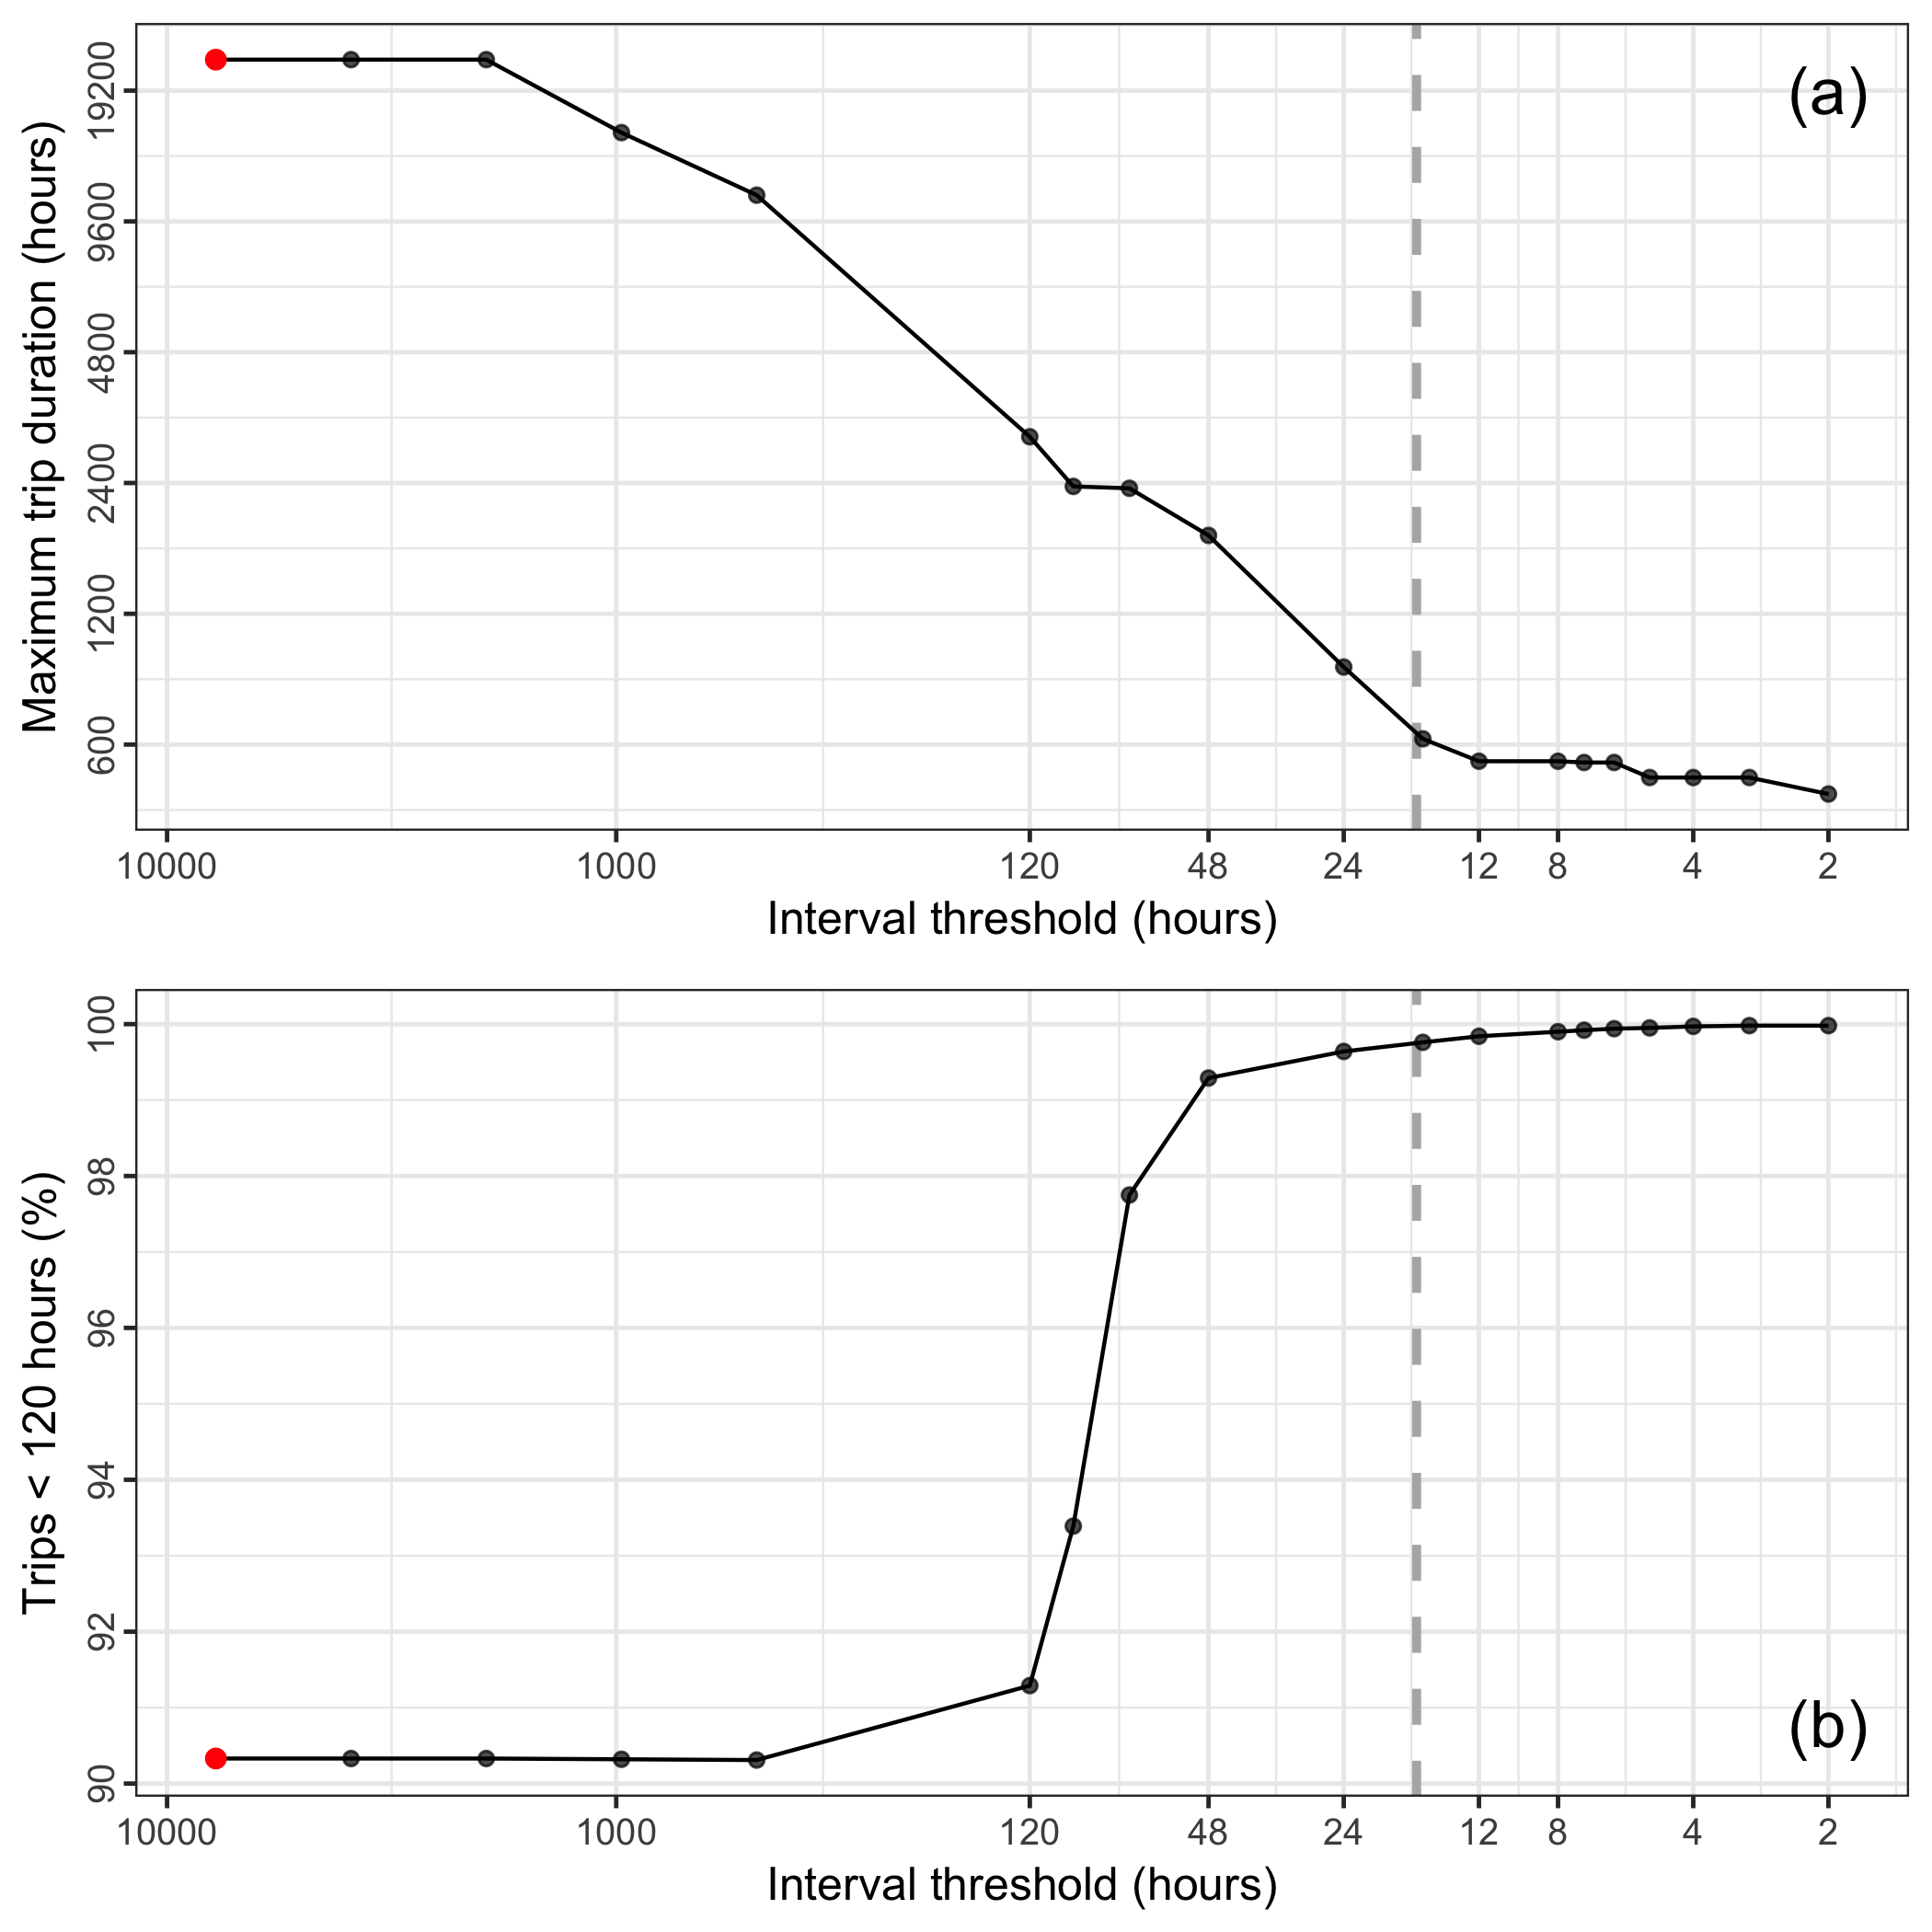
\includegraphics[width=1.00000\textwidth]{../ms_1/ms_1_figs/plot_interval_threshold.png}

\newpage

\subsection{\texorpdfstring{WebFigure 2. Defining impacted vessels based
on the amount of fishing effort inside the Jabuka-Pomo closure one year
prior to the trawling ban. Per vessel fishing effort inside the closure,
as a percentage of total vessel effort, is plotted against vessel
fishing hours inside the closure. Impacted vessels were defined as those
vessels whose total fishing effort (as a percentage and as total hours)
was greater than the 95\textsuperscript{th}
percentile.}{WebFigure 2. Defining impacted vessels based on the amount of fishing effort inside the Jabuka-Pomo closure one year prior to the trawling ban. Per vessel fishing effort inside the closure, as a percentage of total vessel effort, is plotted against vessel fishing hours inside the closure. Impacted vessels were defined as those vessels whose total fishing effort (as a percentage and as total hours) was greater than the 95th percentile.}}\label{webfigure-2.-defining-impacted-vessels-based-on-the-amount-of-fishing-effort-inside-the-jabuka-pomo-closure-one-year-prior-to-the-trawling-ban.-per-vessel-fishing-effort-inside-the-closure-as-a-percentage-of-total-vessel-effort-is-plotted-against-vessel-fishing-hours-inside-the-closure.-impacted-vessels-were-defined-as-those-vessels-whose-total-fishing-effort-as-a-percentage-and-as-total-hours-was-greater-than-the-95th-percentile.}

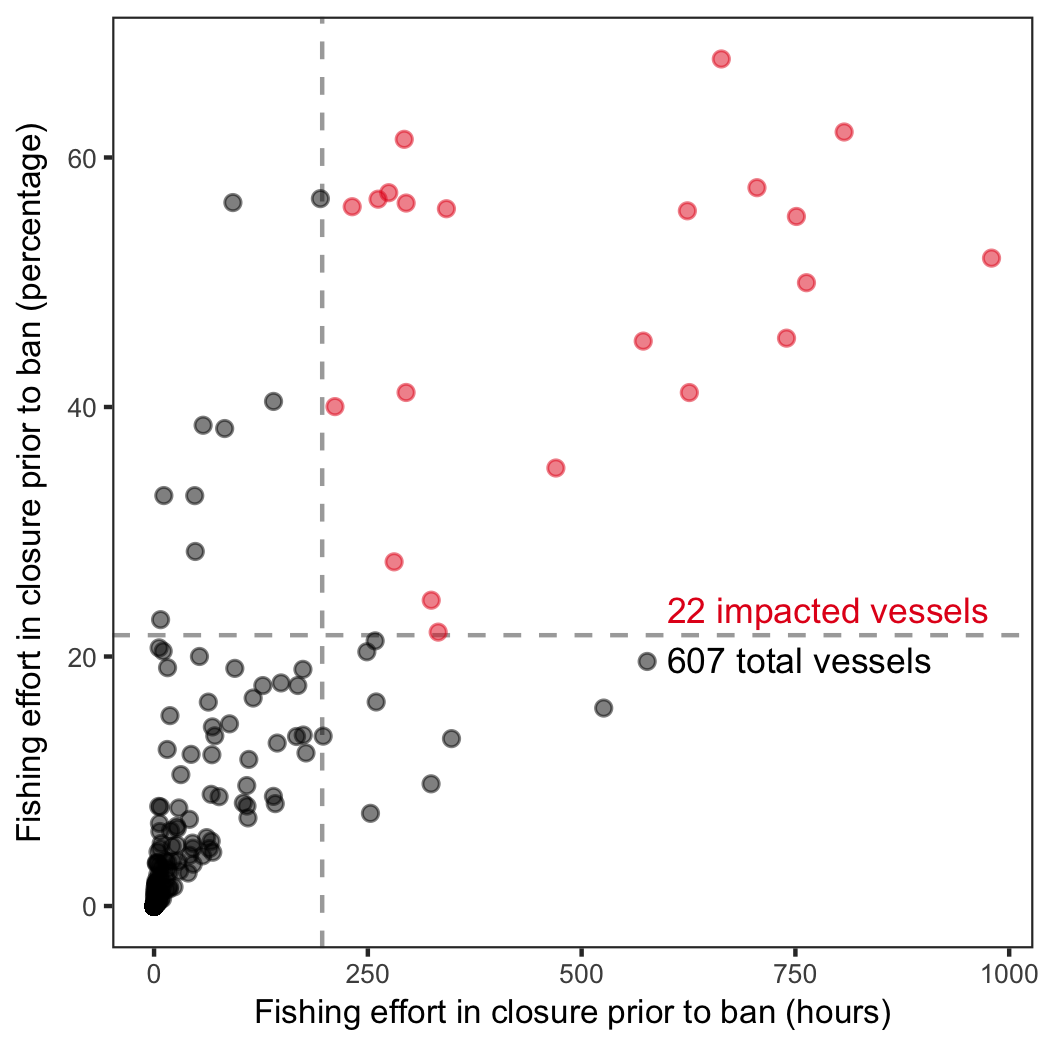
\includegraphics[width=1.00000\textwidth]{../workspace/process_effort_figs/displacement_threshold_scatter.png}

\newpage

\subsection{\texorpdfstring{WebFigure 3. Frequency distribution of
fishing observations by distance from the Jabuka-Pomo border for
impacted vessels (n = 22). The red dashed line represents the threshold
used to exclude fishing observations for impacted vessels, and the blue
dashed line represents the 99.9\textsuperscript{th} percentile for
illustration.}{WebFigure 3. Frequency distribution of fishing observations by distance from the Jabuka-Pomo border for impacted vessels (n = 22). The red dashed line represents the threshold used to exclude fishing observations for impacted vessels, and the blue dashed line represents the 99.9th percentile for illustration.}}\label{webfigure-3.-frequency-distribution-of-fishing-observations-by-distance-from-the-jabuka-pomo-border-for-impacted-vessels-n-22.-the-red-dashed-line-represents-the-threshold-used-to-exclude-fishing-observations-for-impacted-vessels-and-the-blue-dashed-line-represents-the-99.9th-percentile-for-illustration.}

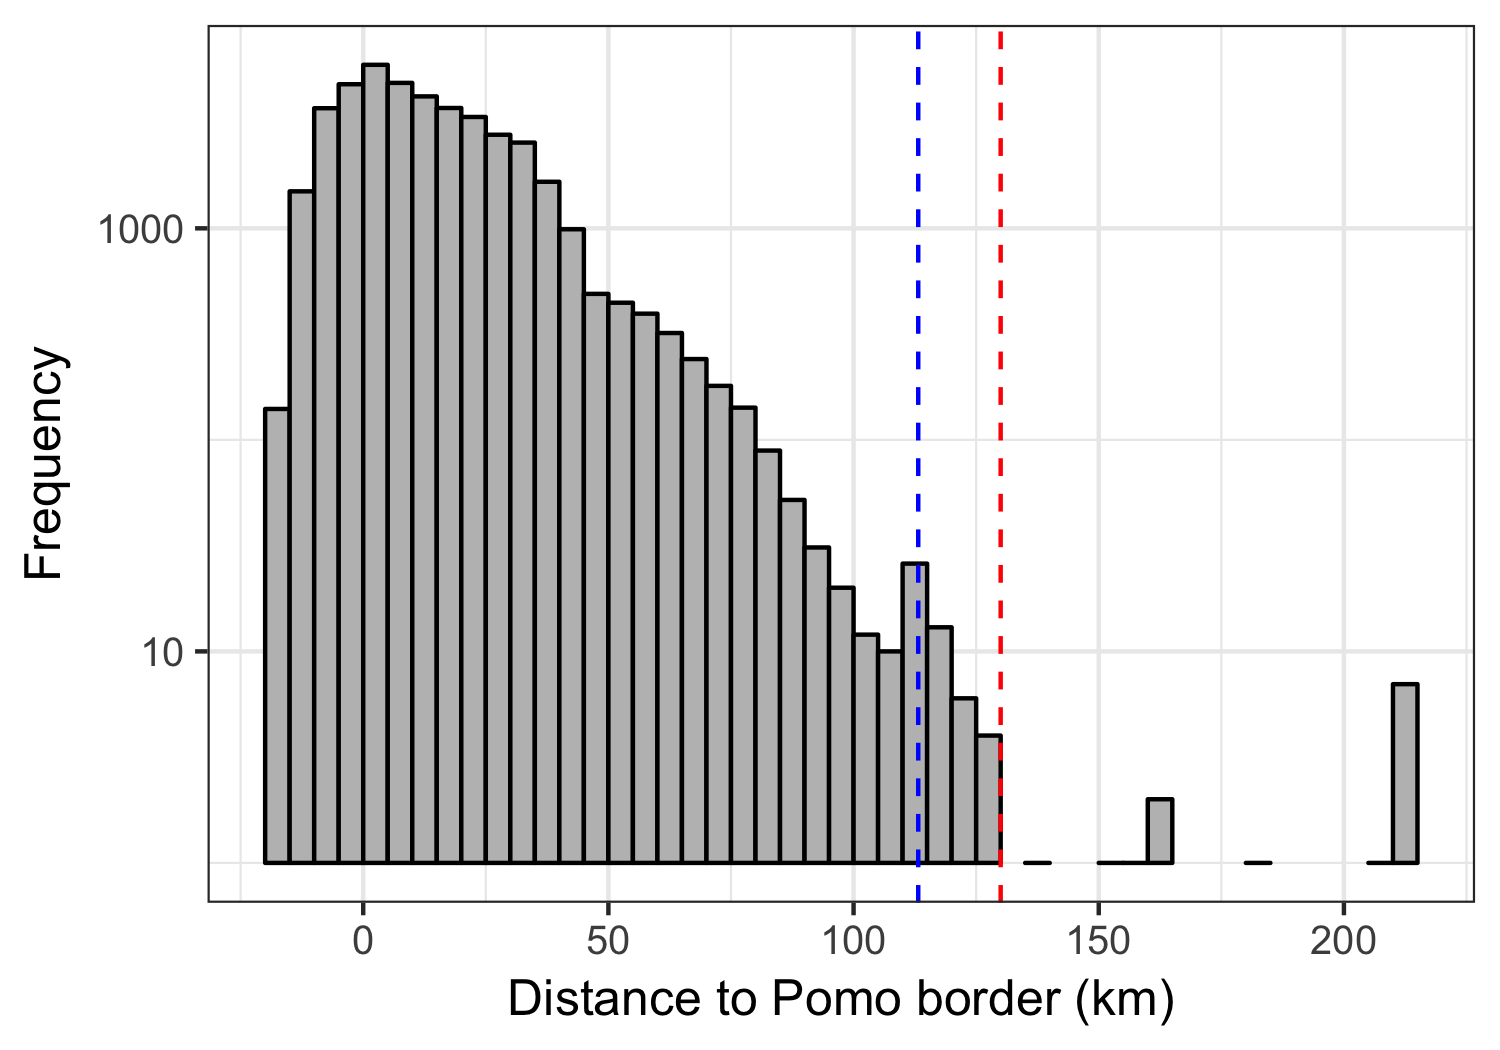
\includegraphics[width=0.90000\textwidth]{../workspace/process_effort_figs/impacted_ves_dist_pomo_histo.png}

\newpage

\subsection{WebFigure 4. Fishing effort of impacted vessels (n = 22)
before and after the cessation of trawling in the Jabuka-Pomo closure
(represented by the inner black polygon). The outer black polygon
represents the defined study area, which do not include fishing
observations \textgreater{} 130km from the Jabuka-Pomo
border.}\label{webfigure-4.-fishing-effort-of-impacted-vessels-n-22-before-and-after-the-cessation-of-trawling-in-the-jabuka-pomo-closure-represented-by-the-inner-black-polygon.-the-outer-black-polygon-represents-the-defined-study-area-which-do-not-include-fishing-observations-130km-from-the-jabuka-pomo-border.}

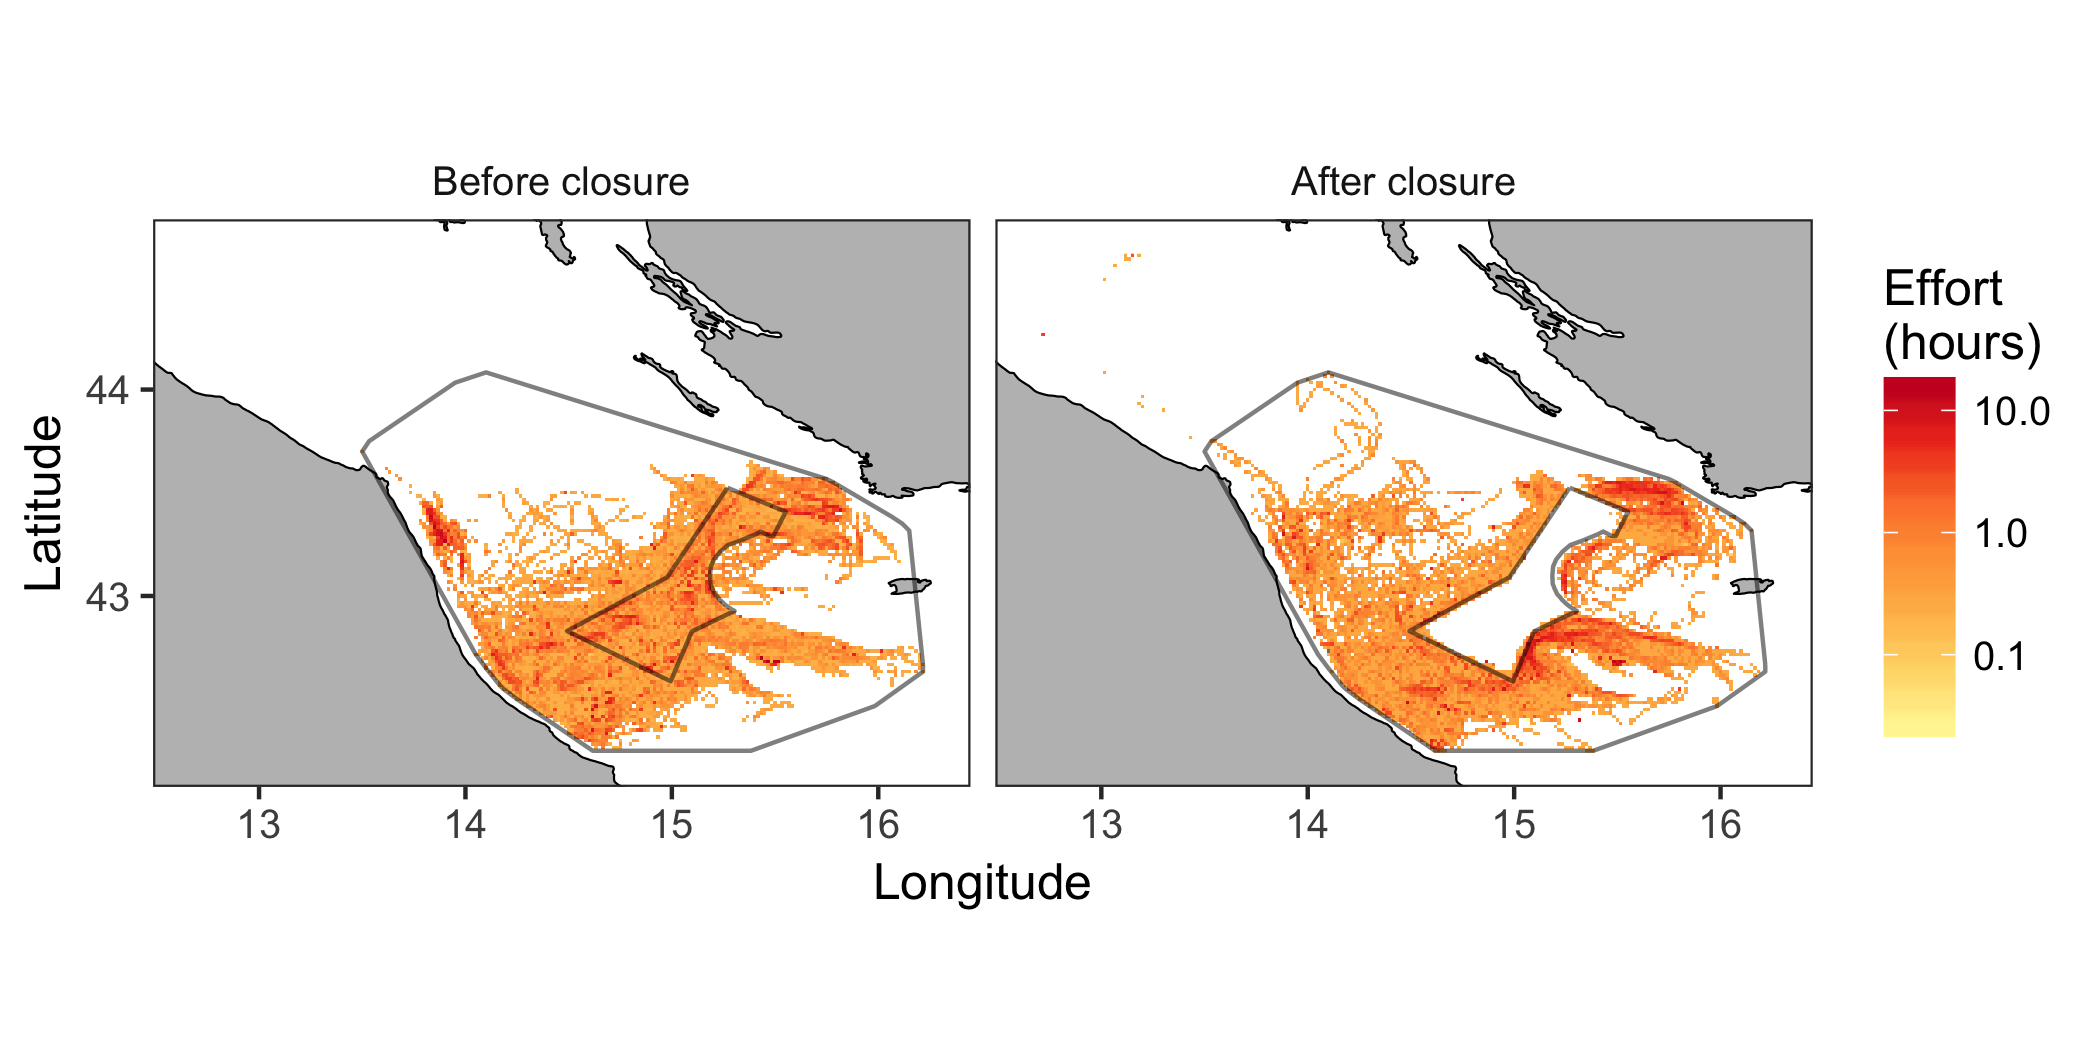
\includegraphics[width=0.90000\textwidth]{../workspace/process_effort_figs/map_impacted_aggregate.png}

\newpage

\subsection{WebFigure 5. Defining the study area and visualizing the
spatial distribution of total fishing effort before and after the
Jabuka-Pomo closure (inner black polygon) summed across three types of
vessels - control, impacted, and other. The outer convex hull polygon
was defined by the maximum distance impacted vessels fished from the
border of the Jabuka-Pomo closure (see WebPanel 1 - Methods - for more
details).}\label{webfigure-5.-defining-the-study-area-and-visualizing-the-spatial-distribution-of-total-fishing-effort-before-and-after-the-jabuka-pomo-closure-inner-black-polygon-summed-across-three-types-of-vessels---control-impacted-and-other.-the-outer-convex-hull-polygon-was-defined-by-the-maximum-distance-impacted-vessels-fished-from-the-border-of-the-jabuka-pomo-closure-see-webpanel-1---methods---for-more-details.}

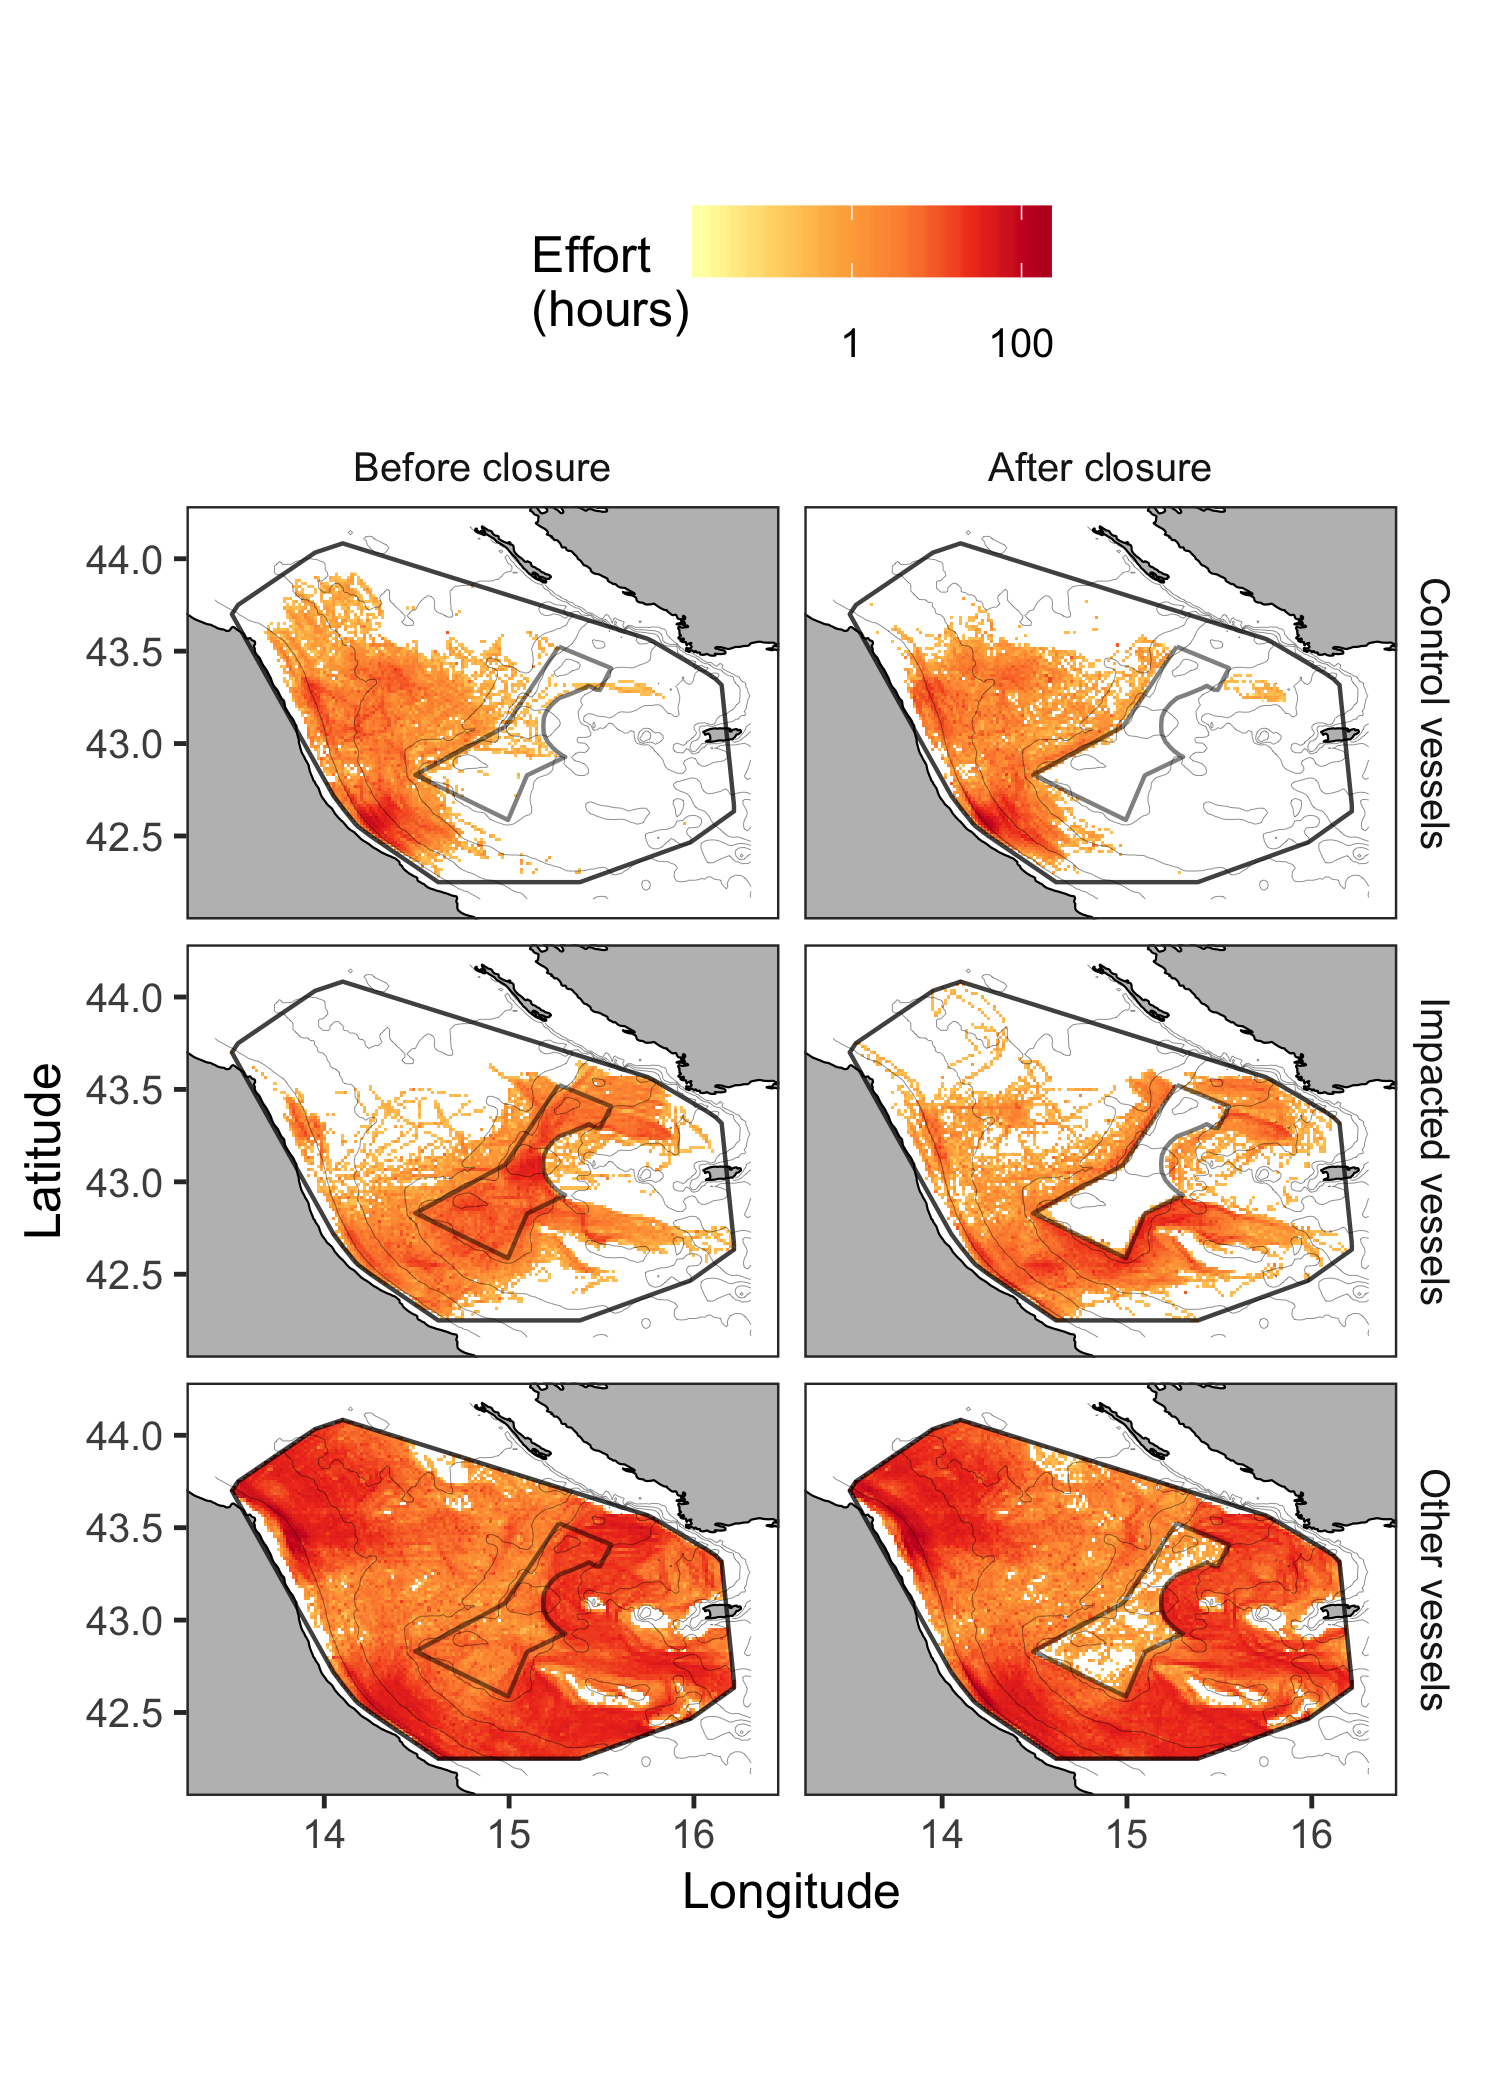
\includegraphics[width=0.90000\textwidth]{../ms_1/ms_1_figs/map_baci_hrs_vesci.png}

\newpage

\subsection{WebFigure 6. Maps of predictors used in the generalized
additivel model. The units of distance variables, depth, and bottom
slope are km, m, and degrees,
respectively.}\label{webfigure-6.-maps-of-predictors-used-in-the-generalized-additivel-model.-the-units-of-distance-variables-depth-and-bottom-slope-are-km-m-and-degrees-respectively.}

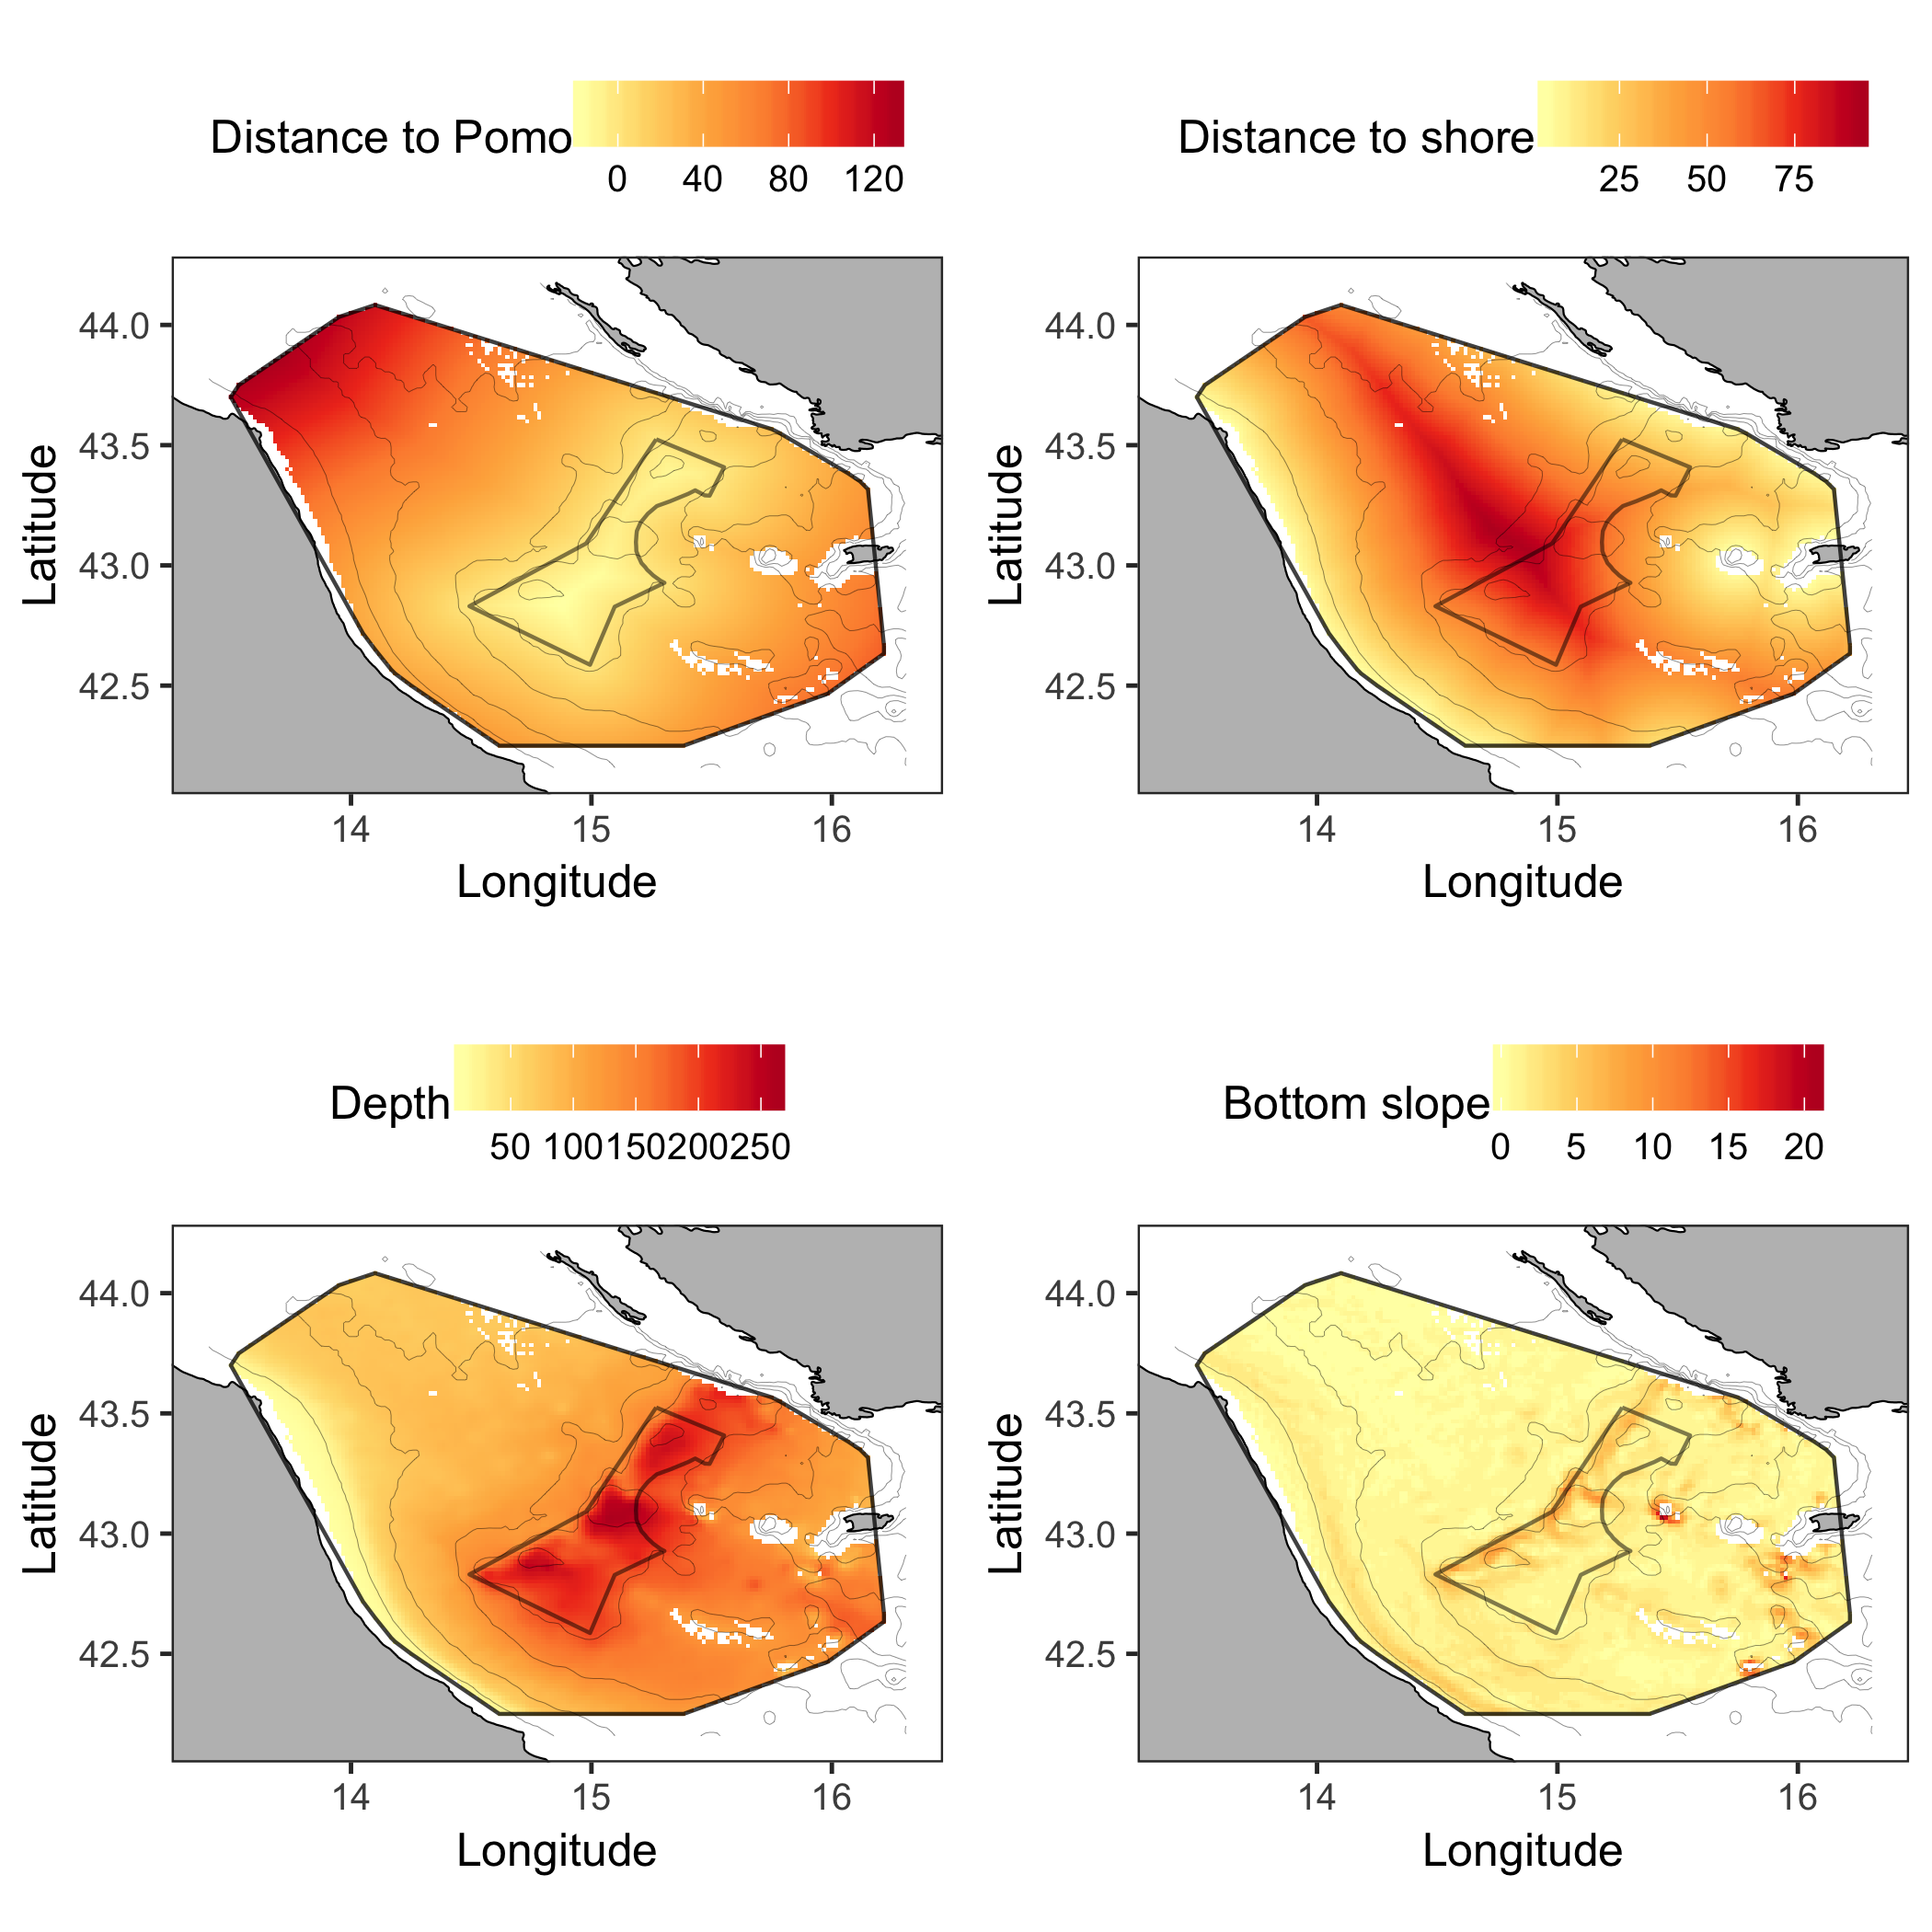
\includegraphics[width=1.00000\textwidth]{../ms_1/ms_1_figs/map_predictors.png}

\newpage

\subsection{WebFigure 7. Maps of nursery persistence for each of five
commercial species; habitat quality is the sum of persistence across all
five species (see WebPanel 1 - Methods - for more details). Habitat
quality was used as a linear predictor in the generalized additive
model.}\label{webfigure-7.-maps-of-nursery-persistence-for-each-of-five-commercial-species-habitat-quality-is-the-sum-of-persistence-across-all-five-species-see-webpanel-1---methods---for-more-details.-habitat-quality-was-used-as-a-linear-predictor-in-the-generalized-additive-model.}

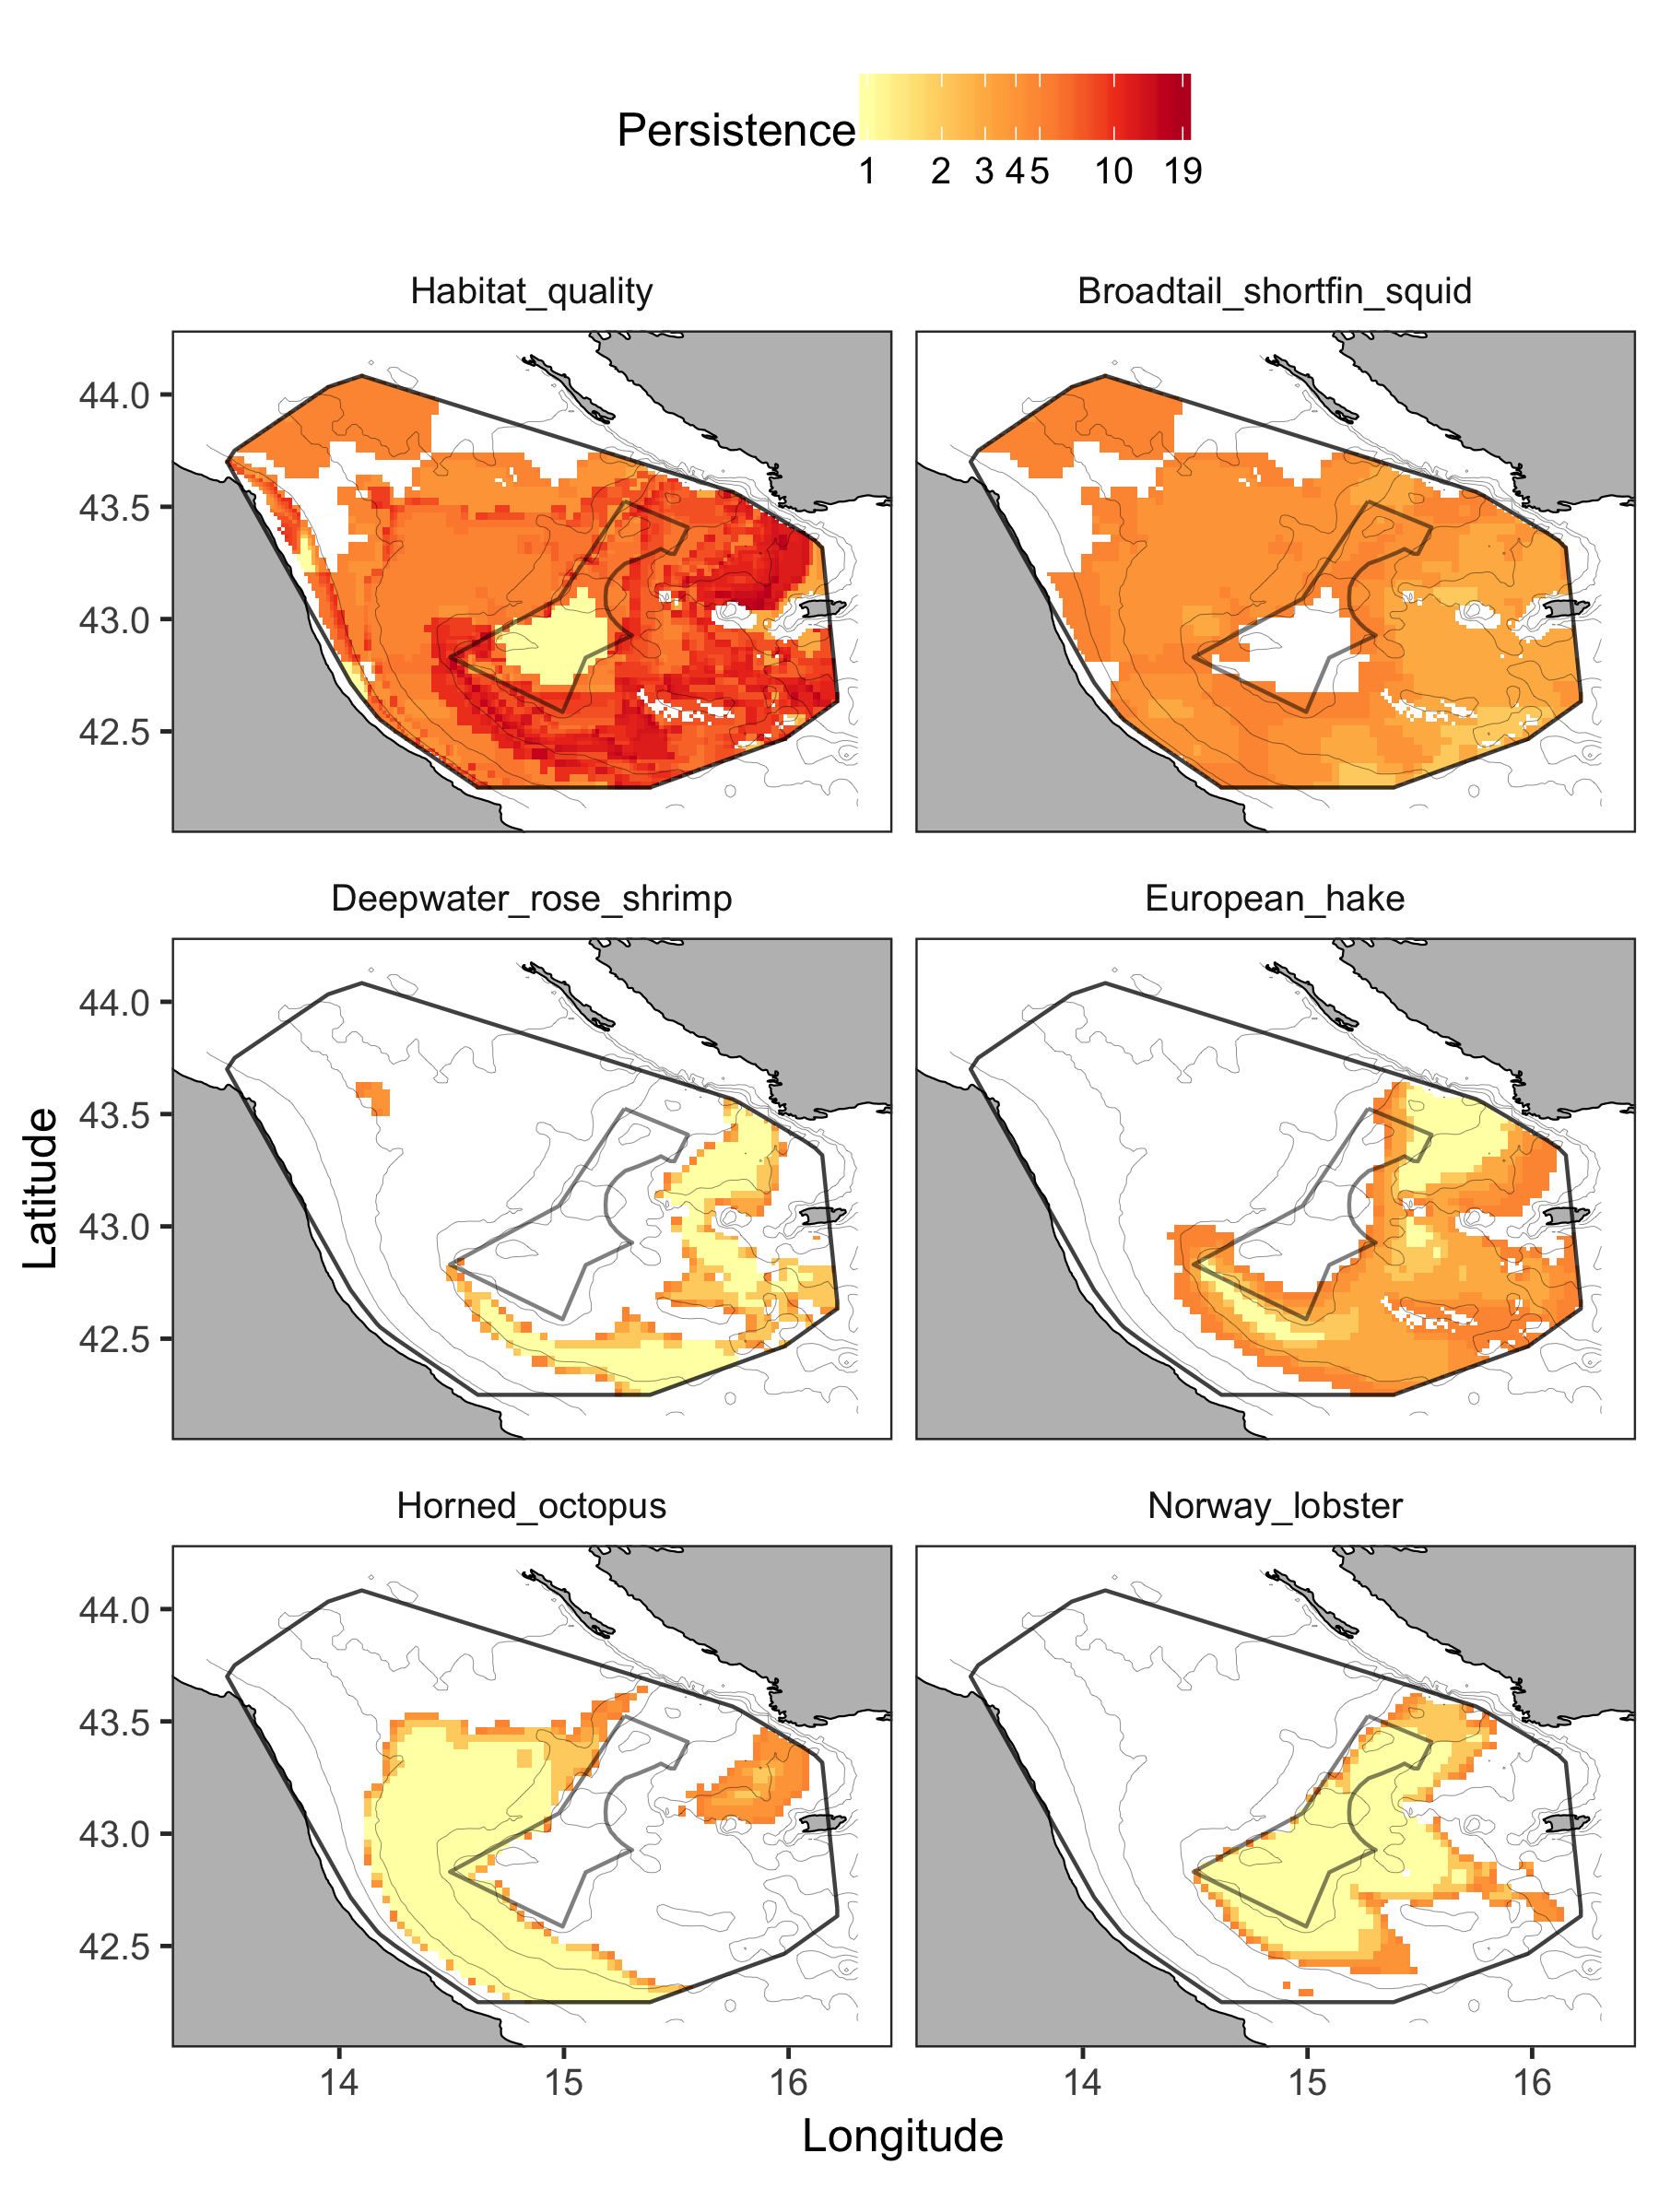
\includegraphics[width=0.90000\textwidth]{../ms_1/ms_1_figs/map_nurseries.png}

\newpage

\subsection{WebFigure 8. Correlation matrix of the predictors used in
the generalized additive
model.}\label{webfigure-8.-correlation-matrix-of-the-predictors-used-in-the-generalized-additive-model.}

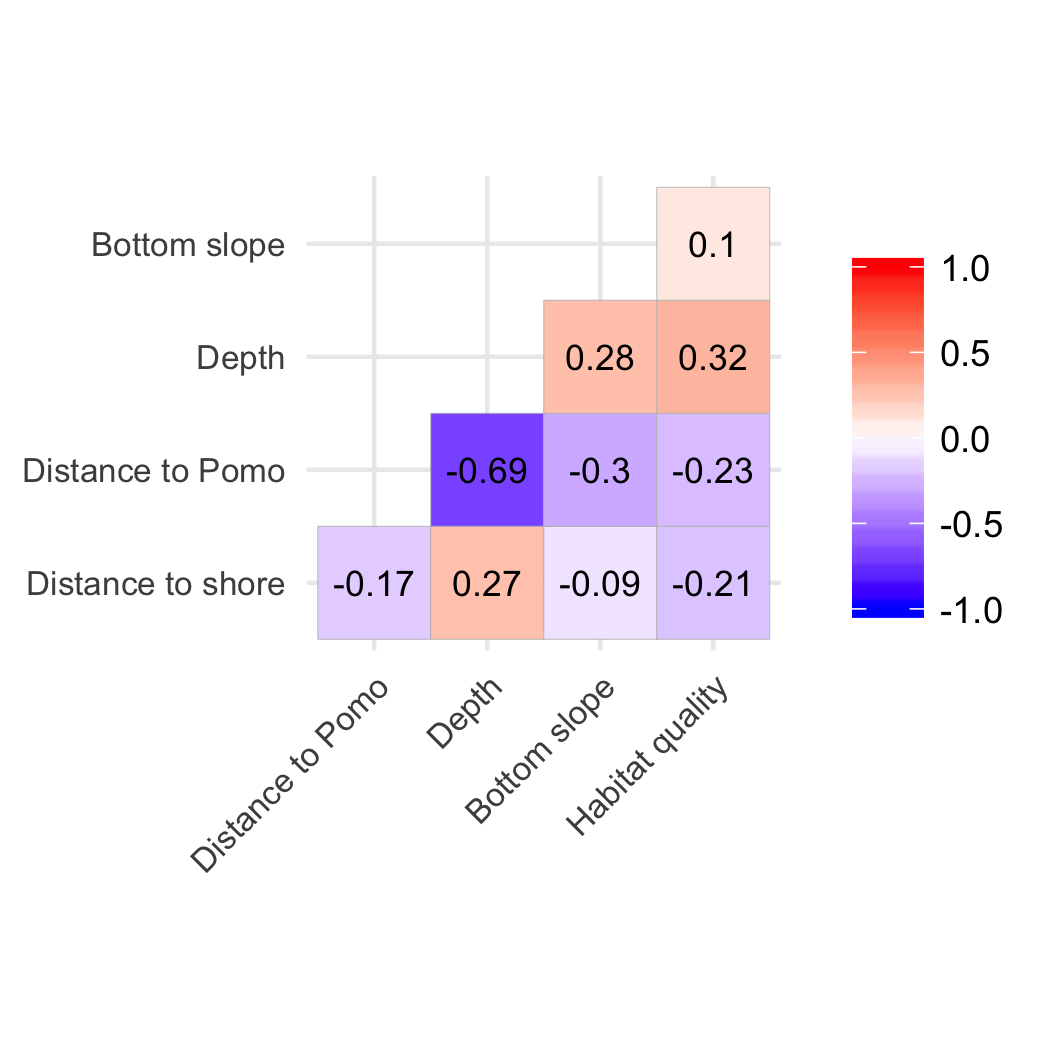
\includegraphics[width=1.00000\textwidth]{../ms_1/ms_1_figs/plot_corr_matrix.png}

\newpage

\subsection{WebFigure 9. Spline correlogram displaying the spatial
autocorrelation of the residuals of the generalized additive model.
Beyond 10km, spatial autocorrelation is
minimal.}\label{webfigure-9.-spline-correlogram-displaying-the-spatial-autocorrelation-of-the-residuals-of-the-generalized-additive-model.-beyond-10km-spatial-autocorrelation-is-minimal.}

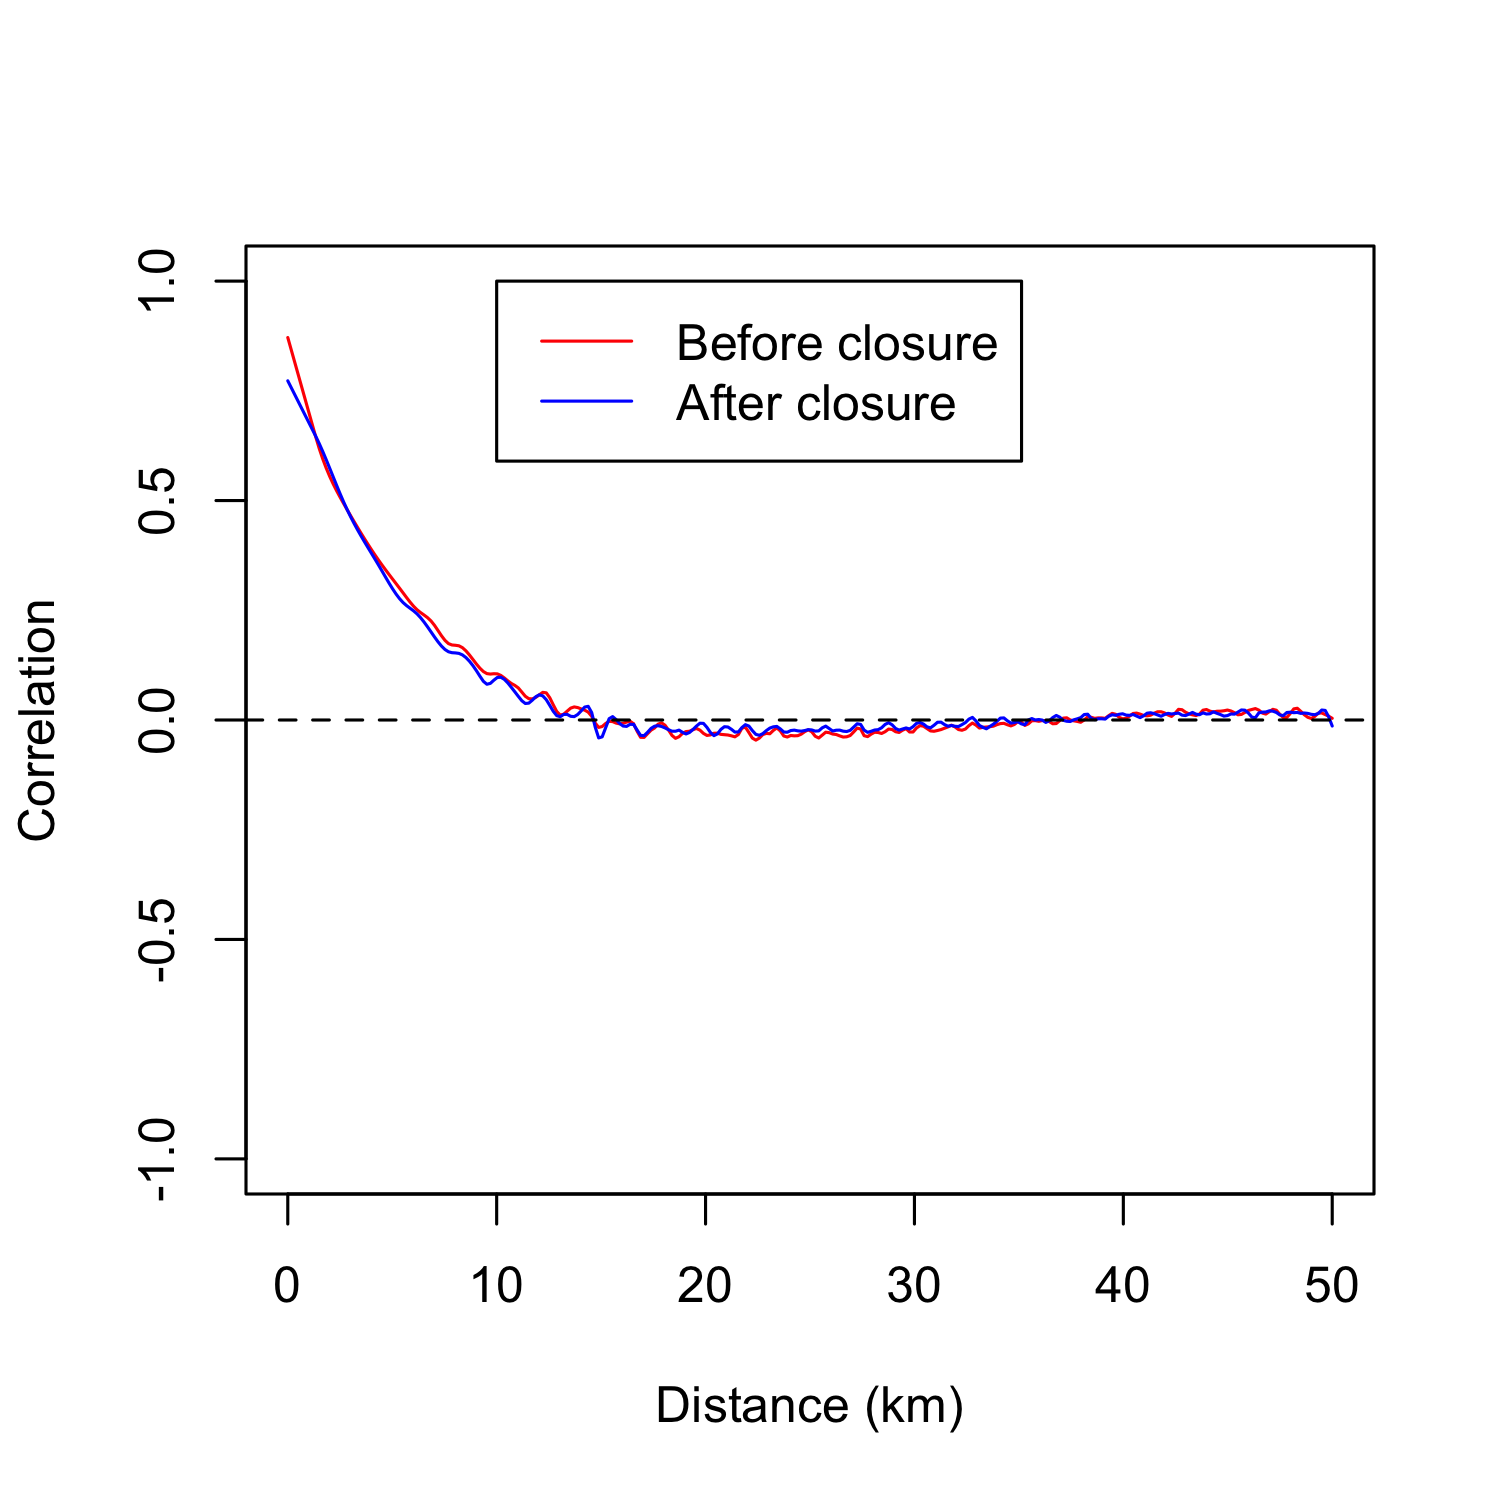
\includegraphics[width=1.00000\textwidth]{../ms_1/ms_1_figs/plot_correlogram.png}

\newpage

\subsection{WebFigure 10. Estimated partial contribution to effort for
smoothed (a, b) and linear (c, d) terms from the generalized additive
model of fishing hours (with 95\% confidence intervals) before and after
the cessation of trawling in the Jabuka-Pomo closure (Table 1). In (a),
the dashed line at 0 indicates the border of the Jabuka-Pomo closure,
such that positive distances are outside the closure and negative
distances are inside the
closure.}\label{webfigure-10.-estimated-partial-contribution-to-effort-for-smoothed-a-b-and-linear-c-d-terms-from-the-generalized-additive-model-of-fishing-hours-with-95-confidence-intervals-before-and-after-the-cessation-of-trawling-in-the-jabuka-pomo-closure-table-1.-in-a-the-dashed-line-at-0-indicates-the-border-of-the-jabuka-pomo-closure-such-that-positive-distances-are-outside-the-closure-and-negative-distances-are-inside-the-closure.}

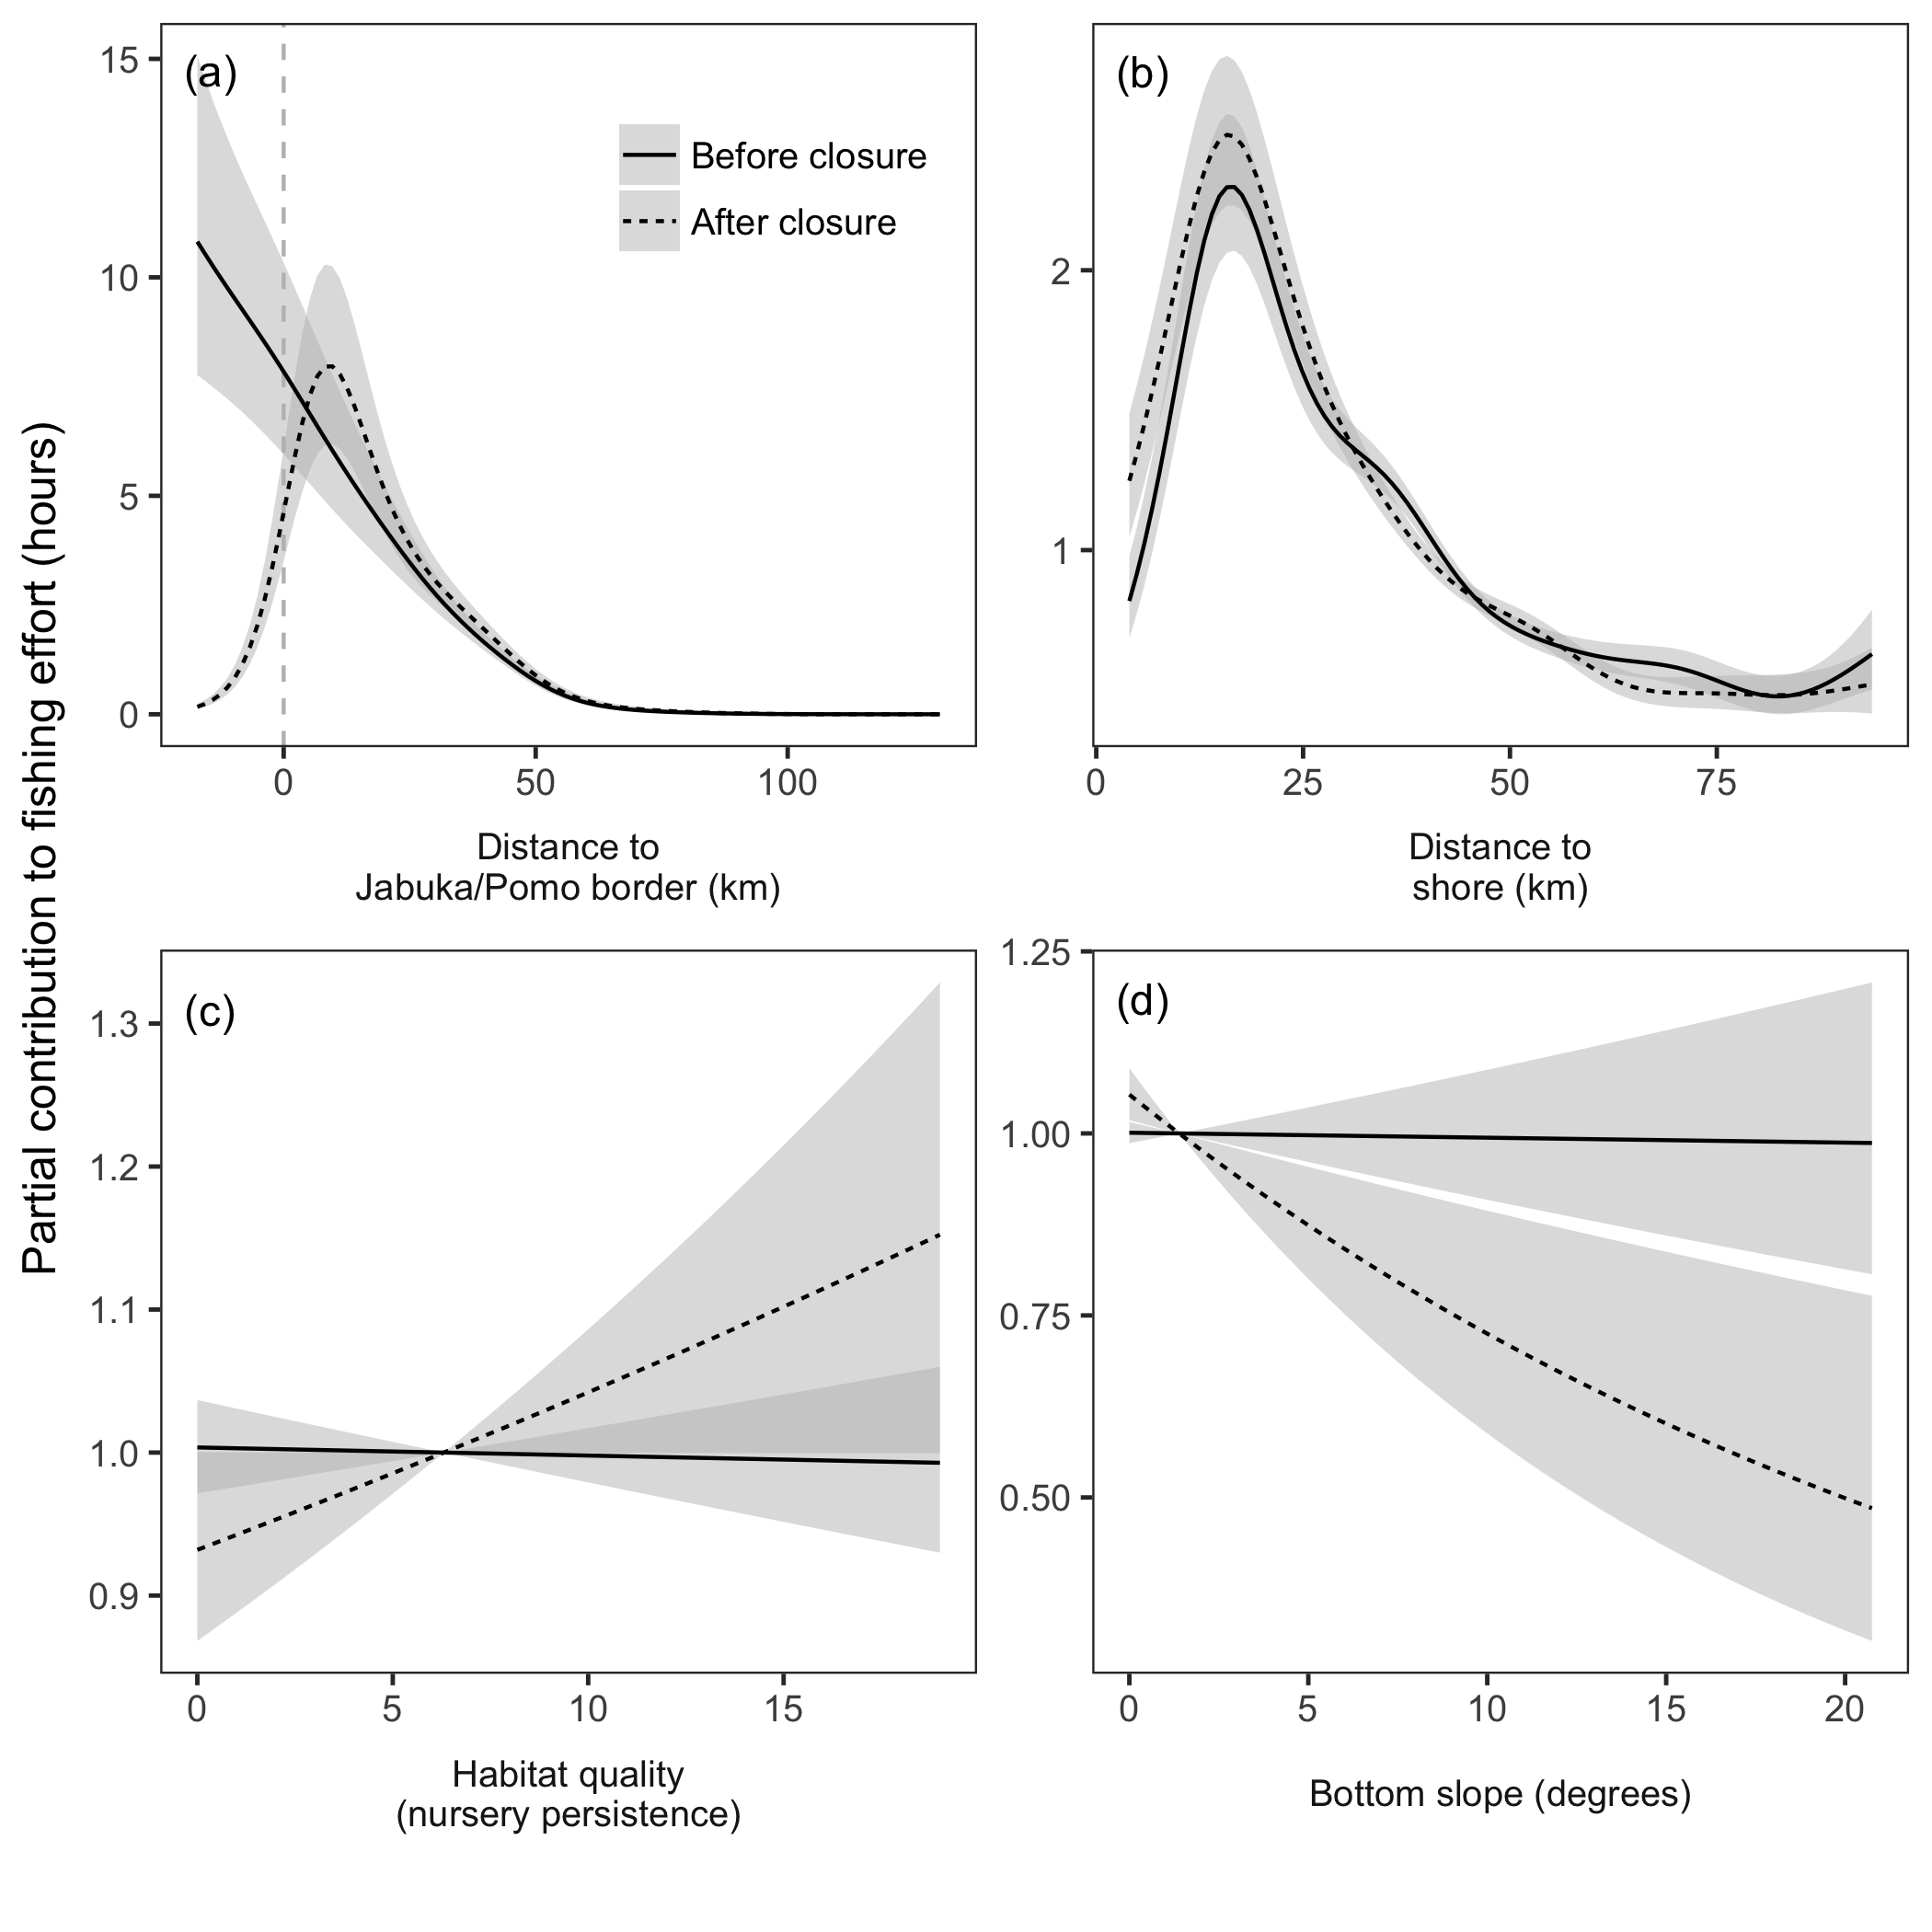
\includegraphics[width=1.00000\textwidth]{../ms_1/ms_1_figs/plot_gam_partials_free_hrs.png}

\newpage

\subsection{WebFigure 11. Monthly time series (January 2014 - July 2016)
of effort inside and outside the Jabuka-Pomo closure, with colors
representing the two nations that fished in the study area. The black
dashed line represents the official start of the trawling ban (25 July
2015), and the gray dashed lines denote the one year periods before and
after the closure used in our analyses. The gray rectangles represent
the annual six week trawling suspension imposed on Italian vessels
during the summer by the Italian Ministry of Agricultural, Food, and
Forestry.}\label{webfigure-11.-monthly-time-series-january-2014---july-2016-of-effort-inside-and-outside-the-jabuka-pomo-closure-with-colors-representing-the-two-nations-that-fished-in-the-study-area.-the-black-dashed-line-represents-the-official-start-of-the-trawling-ban-25-july-2015-and-the-gray-dashed-lines-denote-the-one-year-periods-before-and-after-the-closure-used-in-our-analyses.-the-gray-rectangles-represent-the-annual-six-week-trawling-suspension-imposed-on-italian-vessels-during-the-summer-by-the-italian-ministry-of-agricultural-food-and-forestry.}

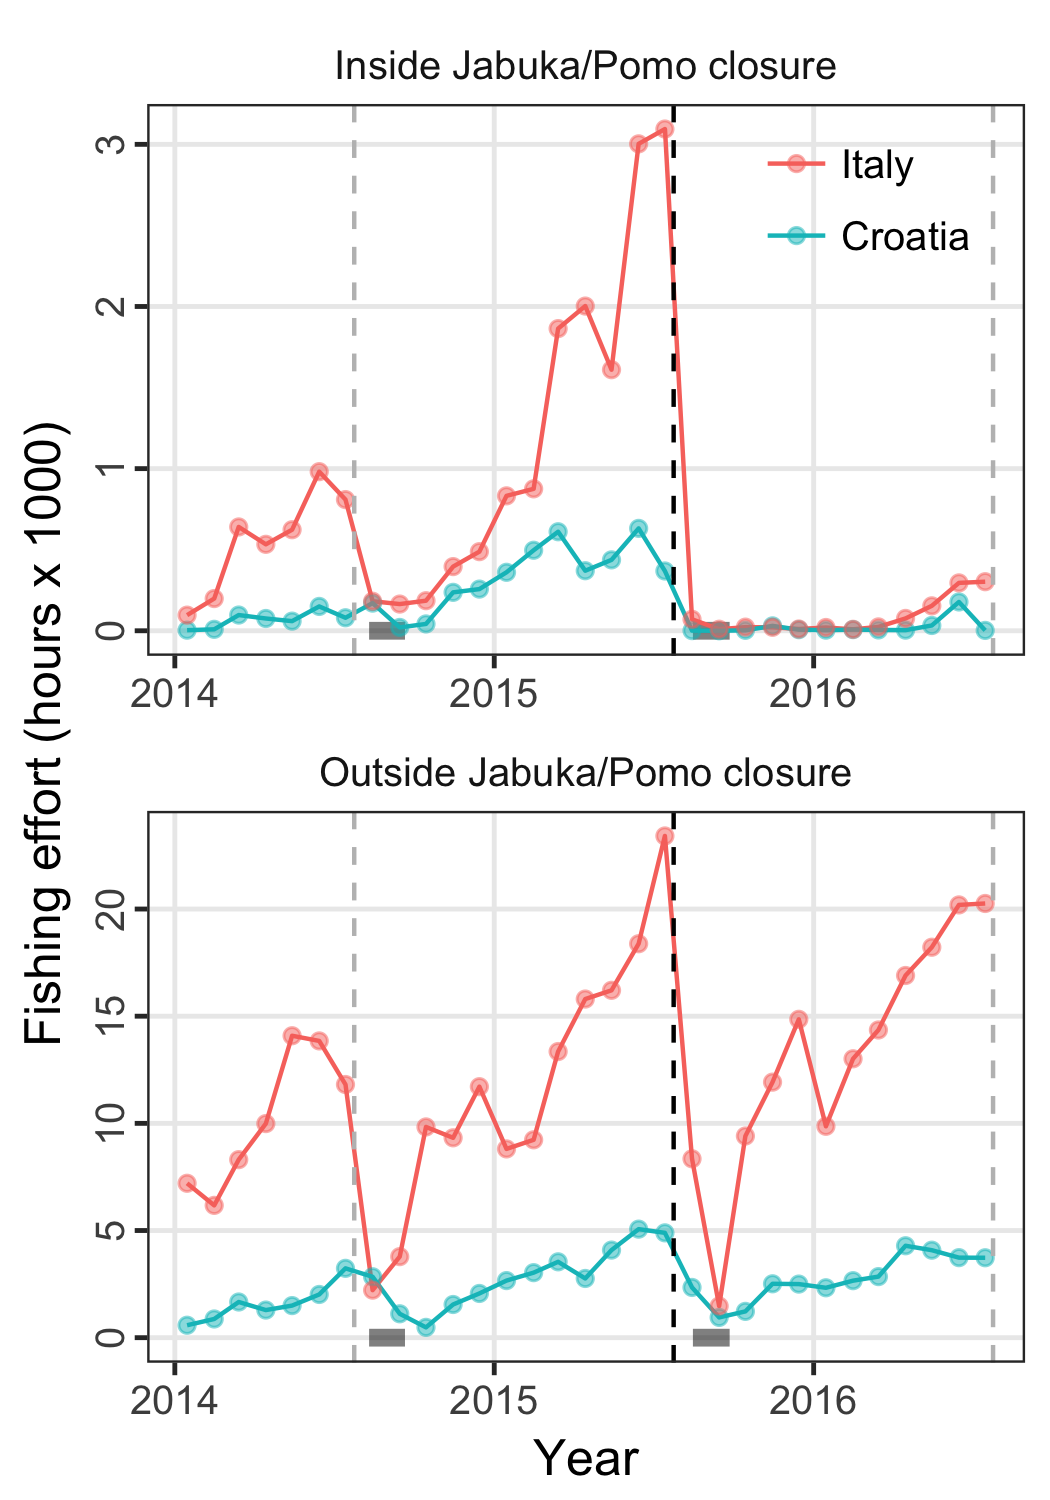
\includegraphics[width=0.75000\textwidth]{../ms_1/ms_1_figs/plot_time_series.png}

\newpage

\subsection{WebFigure 12. Monthly time series (January 2014 - July 2016)
of effort inside the Jabuka-Pomo closure. Each panel represents a unique
vessel, and vessels are arranged in descending order of the total number
of hours fished inside the closure after the trawling ban. Only 22
vessels (of 87) in the upper quartile of total effort inside the closure
after the trawling ban (i.e., \textgreater{} 11.3 hours) are displayed;
these 22 vessels represents 86\% of the incursions (in total hours). The
ports associated with each vessel are listed, with the number of fishing
hours inside the closure after the trawling ban in parentheses. Colors
represent nations, and shapes represent whether vessels were designated
as impacted or other. The black dashed line represents the official
start of the trawling ban (25 July 2015), and the gray dashed lines
denote the one year periods before and after the closure used in our
analyses.}\label{webfigure-12.-monthly-time-series-january-2014---july-2016-of-effort-inside-the-jabuka-pomo-closure.-each-panel-represents-a-unique-vessel-and-vessels-are-arranged-in-descending-order-of-the-total-number-of-hours-fished-inside-the-closure-after-the-trawling-ban.-only-22-vessels-of-87-in-the-upper-quartile-of-total-effort-inside-the-closure-after-the-trawling-ban-i.e.-11.3-hours-are-displayed-these-22-vessels-represents-86-of-the-incursions-in-total-hours.-the-ports-associated-with-each-vessel-are-listed-with-the-number-of-fishing-hours-inside-the-closure-after-the-trawling-ban-in-parentheses.-colors-represent-nations-and-shapes-represent-whether-vessels-were-designated-as-impacted-or-other.-the-black-dashed-line-represents-the-official-start-of-the-trawling-ban-25-july-2015-and-the-gray-dashed-lines-denote-the-one-year-periods-before-and-after-the-closure-used-in-our-analyses.}

\newpage

\subsection{WebFigure 12.}\label{webfigure-12.}

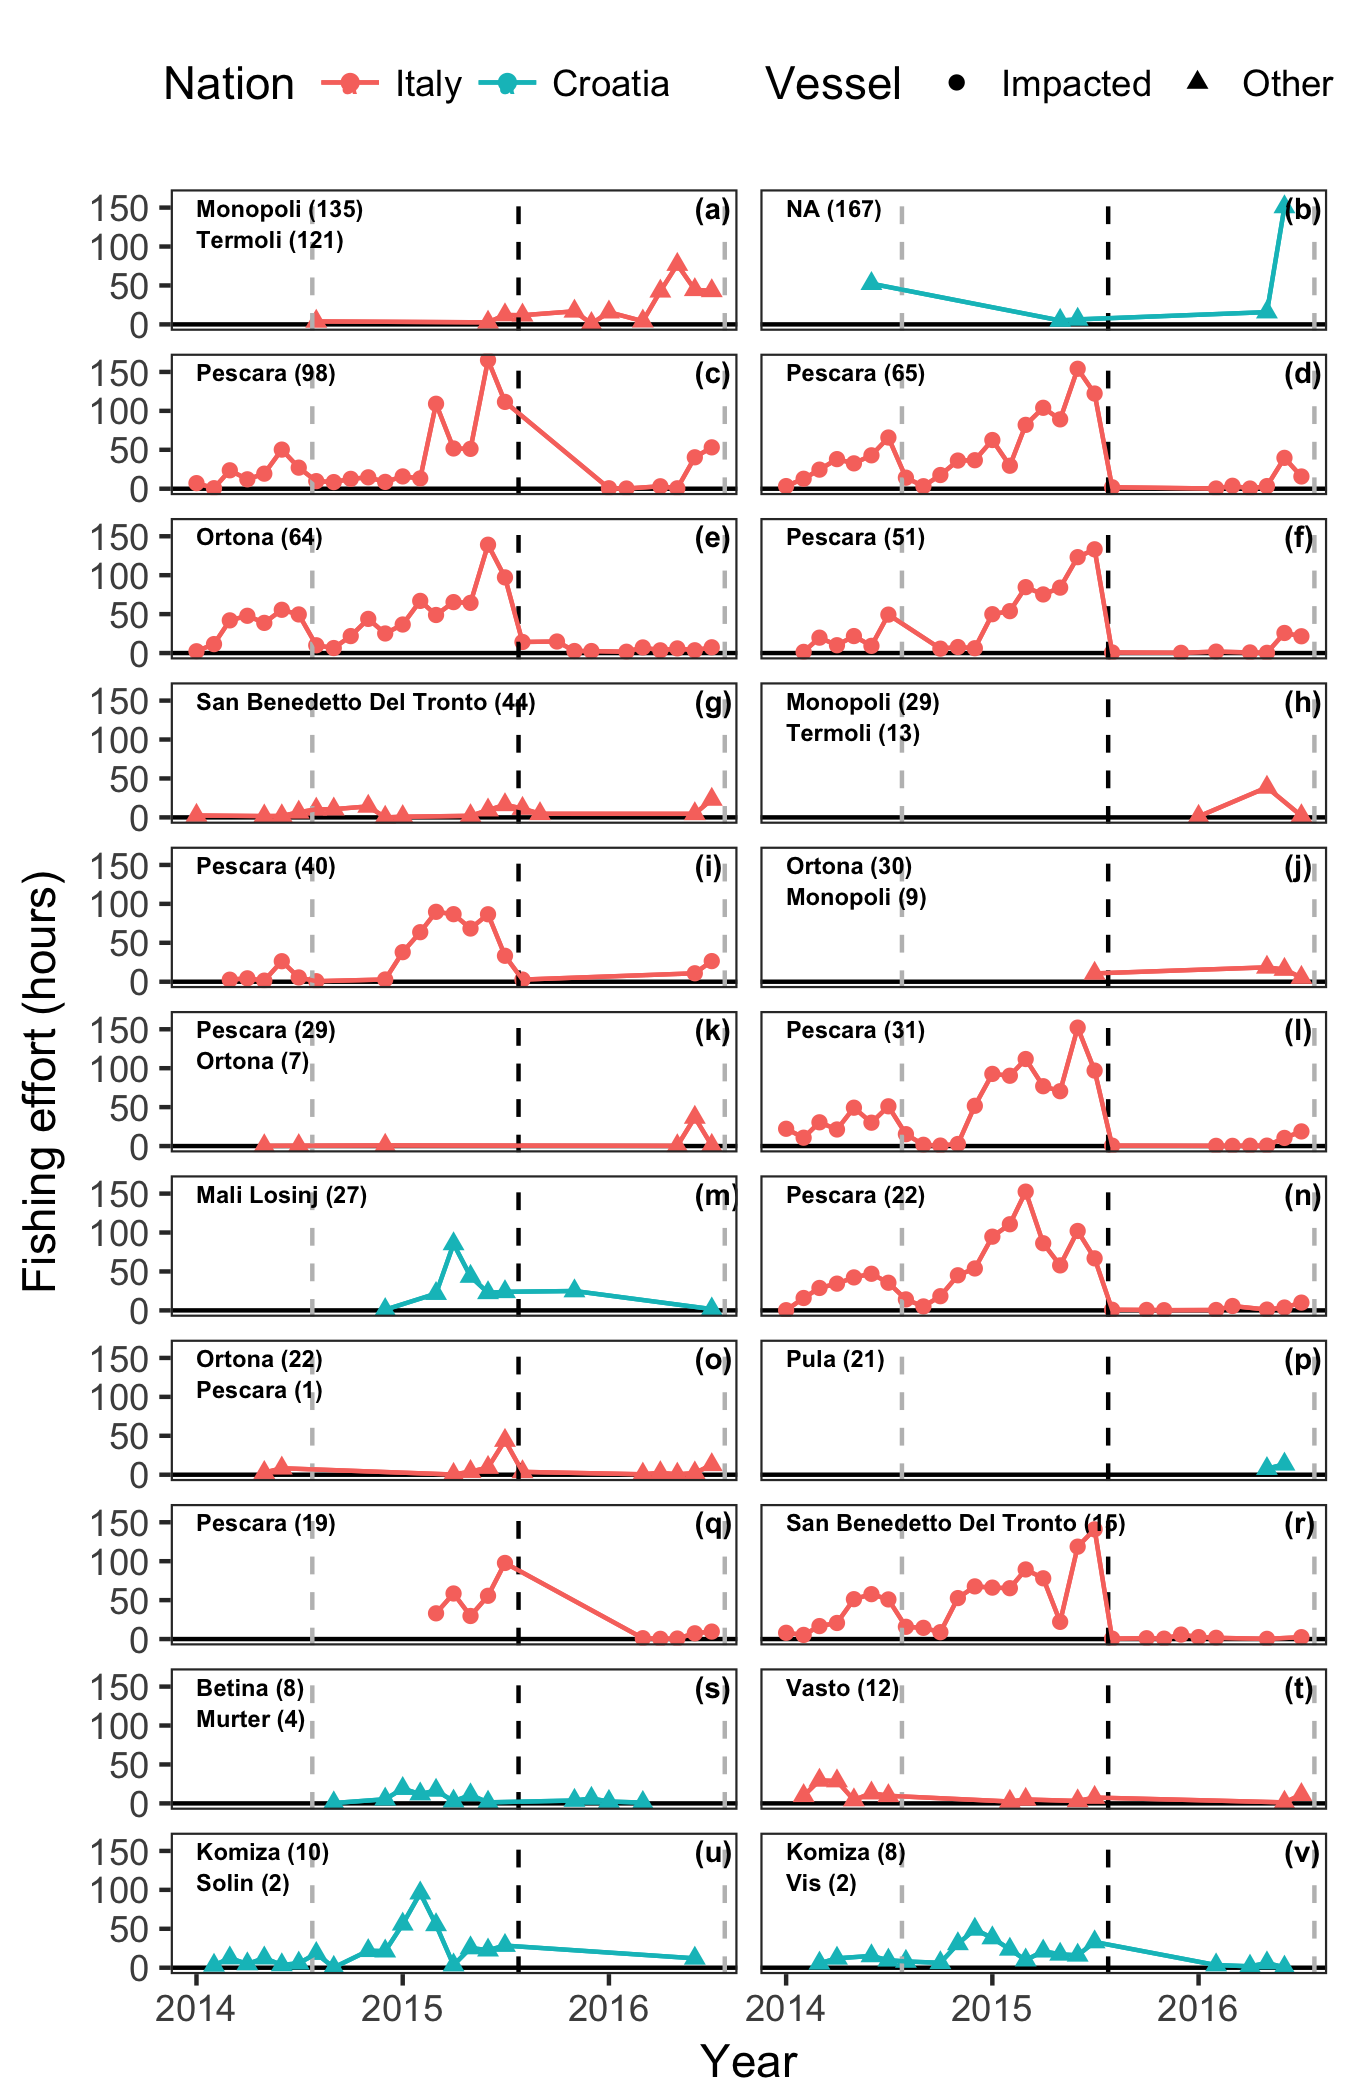
\includegraphics[width=1.00000\textwidth]{../ms_1/ms_1_figs/plot_time_series_incursion_ves_after.png}

\newpage

\subsection{WebFigure 13. Maps of fishing effort for four vessels after
the cessation of trawling in the Jabuka-Pomo closure (represented by the
black polygon). These four maps (a-d) correspond to the vessels in
WebFigure 12 (a-d). The size of points corresponds to the total number
of fishing hours inside the closure associated with each
port.}\label{webfigure-13.-maps-of-fishing-effort-for-four-vessels-after-the-cessation-of-trawling-in-the-jabuka-pomo-closure-represented-by-the-black-polygon.-these-four-maps-a-d-correspond-to-the-vessels-in-webfigure-12-a-d.-the-size-of-points-corresponds-to-the-total-number-of-fishing-hours-inside-the-closure-associated-with-each-port.}

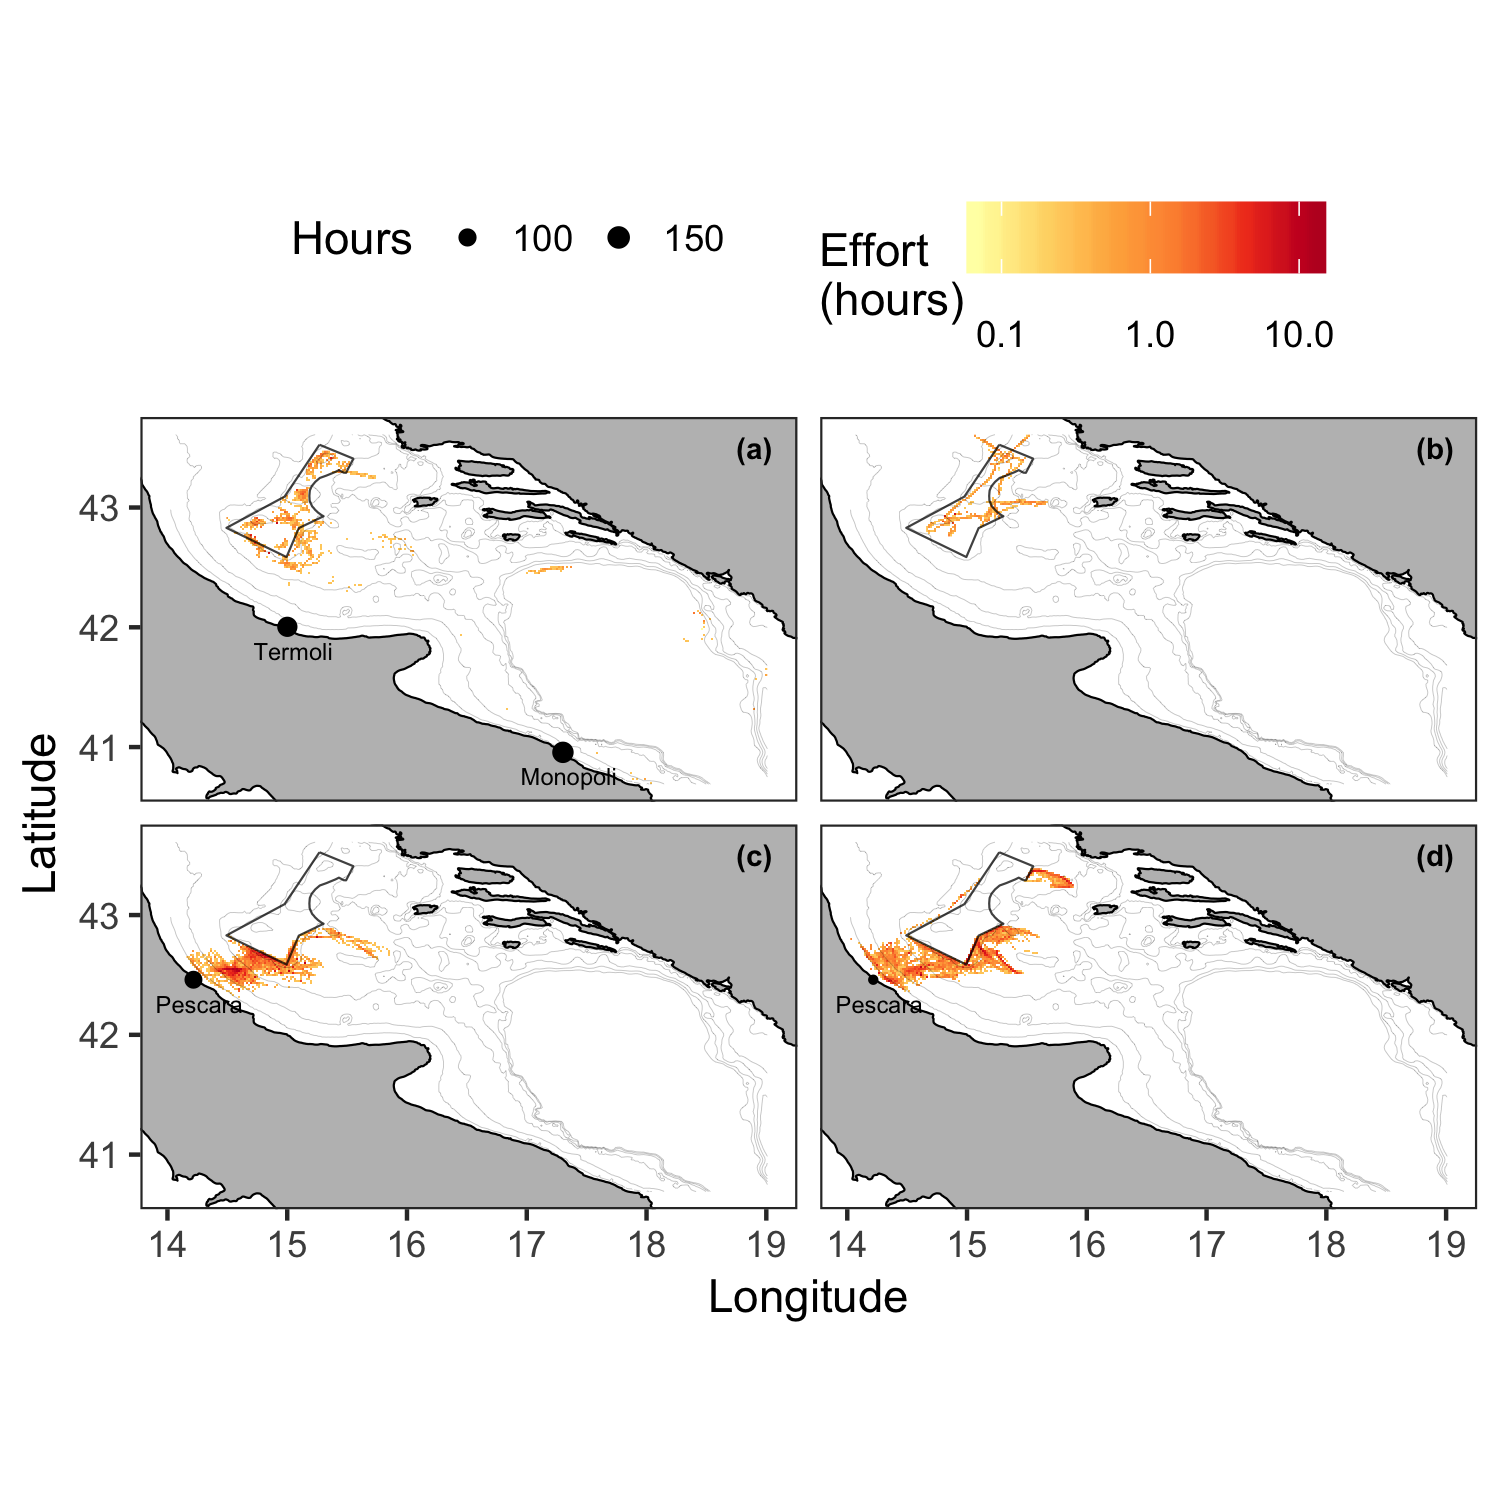
\includegraphics[width=1.00000\textwidth]{../ms_1/ms_1_figs/map_incursions.png}

\newpage

\subsection*{WebReferences}\label{webreferences}
\addcontentsline{toc}{subsection}{WebReferences}

\hypertarget{refs}{}
\hypertarget{ref-bertrand2005levy}{}
Bertrand S, Burgos JM, Gerlotto F, and Atiquipa J. 2005. Lévy
trajectories of Peruvian purse-seiners as an indicator of the spatial
distribution of anchovy (\emph{Engraulis ringens}). \emph{ICES Journal
of Marine Science} \textbf{62}: 477--82.

\hypertarget{ref-colloca2015seascape}{}
Colloca F, Garofalo G, and Bitetto I \emph{et al.} 2015. The seascape of
demersal fish nursery areas in the north Mediterranean sea, a first step
towards the implementation of spatial planning for trawl fisheries.
\emph{PloS One} \textbf{10}: e0119590.

\hypertarget{ref-euro_stat2016}{}
Eurostat. 2016. Fishing fleet by type of gear and engine power.

\hypertarget{ref-hintzen2012vmstools}{}
Hintzen NT, Bastardie F, and Beare D \emph{et al.} 2012. VMStools:
Open-source software for the processing, analysis and visualisation of
fisheries logbook and VMS data. \emph{Fisheries Research} \textbf{115}:
31--43.

\hypertarget{ref-lee2010developing}{}
Lee J, South AB, and Jennings S. 2010. Developing reliable, repeatable,
and accessible methods to provide high-resolution estimates of
fishing-effort distributions from vessel monitoring system (VMS) data.
\emph{ICES Journal of Marine Science} \textbf{67}: 1260--71.

\hypertarget{ref-murawski2005effort}{}
Murawski SA, Wigley SE, and Fogarty MJ \emph{et al.} 2005. Effort
distribution and catch patterns adjacent to temperate MPAs. \emph{ICES
Journal of Marine Science} \textbf{62}: 1150--67.

\hypertarget{ref-rlesc}{}
R Core Team. 2017. R: A language and environment for statistical
computing. Vienna, Austria: R Foundation for Statistical Computing.

\hypertarget{ref-russo2013spatial}{}
Russo T, Parisi A, and Cataudella S. 2013. Spatial indicators of fishing
pressure: Preliminary analyses and possible developments.
\emph{Ecological Indicators} \textbf{26}: 141--53.

\hypertarget{ref-sbrocco2013marspec}{}
Sbrocco EJ and Barber PH. 2013. MARSPEC: Ocean climate layers for marine
spatial ecology. \emph{Ecology} \textbf{94}: 979--9.

\hypertarget{ref-vespe2016mapping}{}
Vespe M, Gibin M, and Alessandrini A \emph{et al.} 2016. Mapping EU
fishing activities using ship tracking data. \emph{Journal of Maps}
\textbf{12}: 520--5.

\hypertarget{ref-wood2006gam}{}
Wood S. 2006. Generalized additive models: An introduction with R.
Chapman; Hall/CRC.

\hypertarget{ref-zuur2010protocol}{}
Zuur AF, Ieno EN, and Elphick CS. 2010. A protocol for data exploration
to avoid common statistical problems. \emph{Methods in Ecology and
Evolution} \textbf{1}: 3--14.


\end{document}
